%!TEX root = ../thesis.tex
%*******************************************************************************
%****************************** Third Chapter **********************************
%*******************************************************************************
\chapter{Data and analysis}

% **************************** Define Graphics Path **************************
\ifpdf
    \graphicspath{{Chapter3/Figs/Raster/}{Chapter3/Figs/PDF/}{Chapter3/Figs/}}
\else
    \graphicspath{{Chapter3/Figs/Vector/}{Chapter3/Figs/}}
\fi

\section[SEM Data]{SEM Data}
\label{section3.1}

\subsection[Azurite and blue verditer]{Azurite and blue verditer}
\label{subsection3.1.1}

This section discusses qualitatively the morphological features, regularity, and approximate particle size of the reference samples described in \textit{Table \ref{table:ref_sample}}. Additional SEM images for all samples that are not discussed here are presented in Appendix A, Supplemental data. The purpose of this work was to establish expectations for particle morphology for natural and synthetic copper carbonate samples. Qualitative analysis of particle appearance as well as quantitative analysis of particle size distributions is presented.


% ************************************************     HKI nat az sample     *******************************************************************

\textit{Figures \ref{fig:hki_nat_az_sem_1} and \ref{fig:hki_nat_az_sem_2}} show the sample HKI natural azurite. This sample is of unknown date and provenance but is confirmed to be naturally produced, which offers a baseline against which to compare other samples known to be synthetic or of unknown origin. Maginification ranges from 250x to 4000x. Significant surface charging was not observed with this sample.

In \textit{Figure \ref{fig:hki_nat_az_sem_1}}, images at 250x and 750x magnification are shown. Particle sizes are very irregular at 250x, as are shapes and volumes. Particles appear to be relatively flat-sided rather than rough. 

It is possible to see the surface texture of larger particles more clearly at 750x magnification in \textit{Figure \ref{fig:hki_nat_az_sem_2}}. It appears that there are smaller particles embedded in or settled on the surface of larger particles, making a rough surface. Particles have clearly sharp angular edges and are not rounded. At this magnification the large variation in particle size is apparent, and the asymmetry of the material is noted. However, the texture on the surface is consistent in size in contrast to the macro-scale heterogeneity.

\begin{figure}[H]
\centering
\begin{minipage}{.45\textwidth}
  \centering
  \includegraphics[width=\linewidth]{HKI_natural_azurite_x250_5_040521}
\end{minipage}
\begin{minipage}{.45\textwidth}
  \centering
  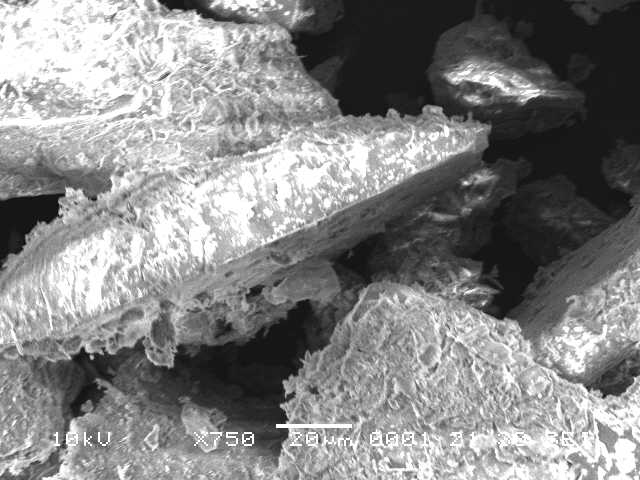
\includegraphics[width=\linewidth]{HKI_natural_azurite_x750_3_040521}
\end{minipage}
\caption[SEM images: Sample HKI, natural azurite]{SEM images: Sample HKI, natural azurite. Magnification: \textbf{left)} 250x, \textbf{right)} 750x.}
\label{fig:hki_nat_az_sem_1}
\end{figure}

\textit{Figure \ref{fig:hki_nat_az_sem_2}} shows images at 2000x and 4000x magnifications. The image on the left, at 2000x, shows clear sharp-sided particles. These are extremely uneven. At very high magnification (4000x), the fine structure of the sample is shown clearly. There is still significant size variation at this magnification, and interesting needle like crystal formations are observed. These do appear to be orientated in some places, possibly showing the areas of crystal nucleation and growth. Other needle like crystals appear randomly orientated. Notably, this ordering is not readily observed in other samples, though needle like crystals are.

\begin{figure}[H]
\centering
\begin{minipage}{.45\textwidth}
  \centering
  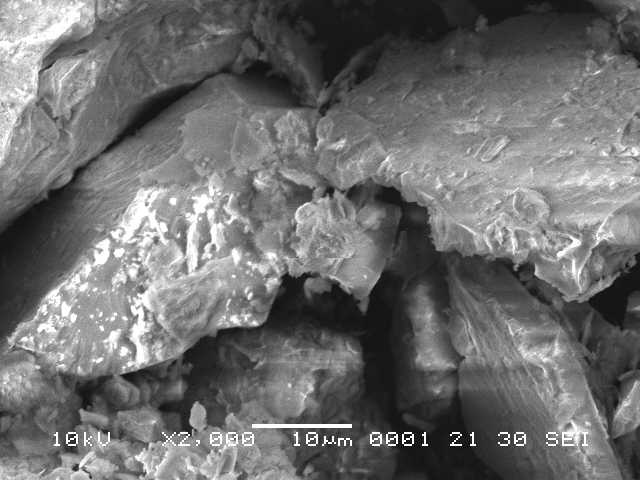
\includegraphics[width=\linewidth]{HKI_natural_azurite_x2000_3_040521}
\end{minipage}
\begin{minipage}{.45\textwidth}
  \centering
  \includegraphics[width=\linewidth]{HKI_natural_azurite_x4000_5_040521}
\end{minipage}
\caption[SEM images: Sample HKI, natural azurite]{SEM images: Sample HKI, natural azurite. Magnification: \textbf{left)} 2000x, \textbf{right)} 4000x.}
\label{fig:hki_nat_az_sem_2}
\end{figure}


% ************************************************     Az1     *******************************************************************

Sample Az1, likely from a natural source, is shown in \textit{Figure \ref{fig:az1_sem_1}}. 

\textit{Figure \ref{fig:az1_sem_1}}, shows sample Az1 at 750x magnification (left) and 2000x magnification (right). The 750x image shows significant size variation in the sample. There are many flat, sharp particles as well as many smaller particles. It is difficult to determine whether the larger pieces of sample are aggregates of smaller particles or larger intact pieces; the surfaces of these appear almost pocked.

At 2000x, the image shows the flat edge of a larger particle. There is a great deal of surface texture, as well as some intriguing grid formations that do not appear to be artifacts of the SEM. These may be due to grinding and polishing of the pigment, but also may suggest some crytal ordering. Uniformity of shape and size is low at all magnifications and all over the sample.

\begin{figure}[H]
\centering
\begin{minipage}{.45\textwidth}
  \centering
  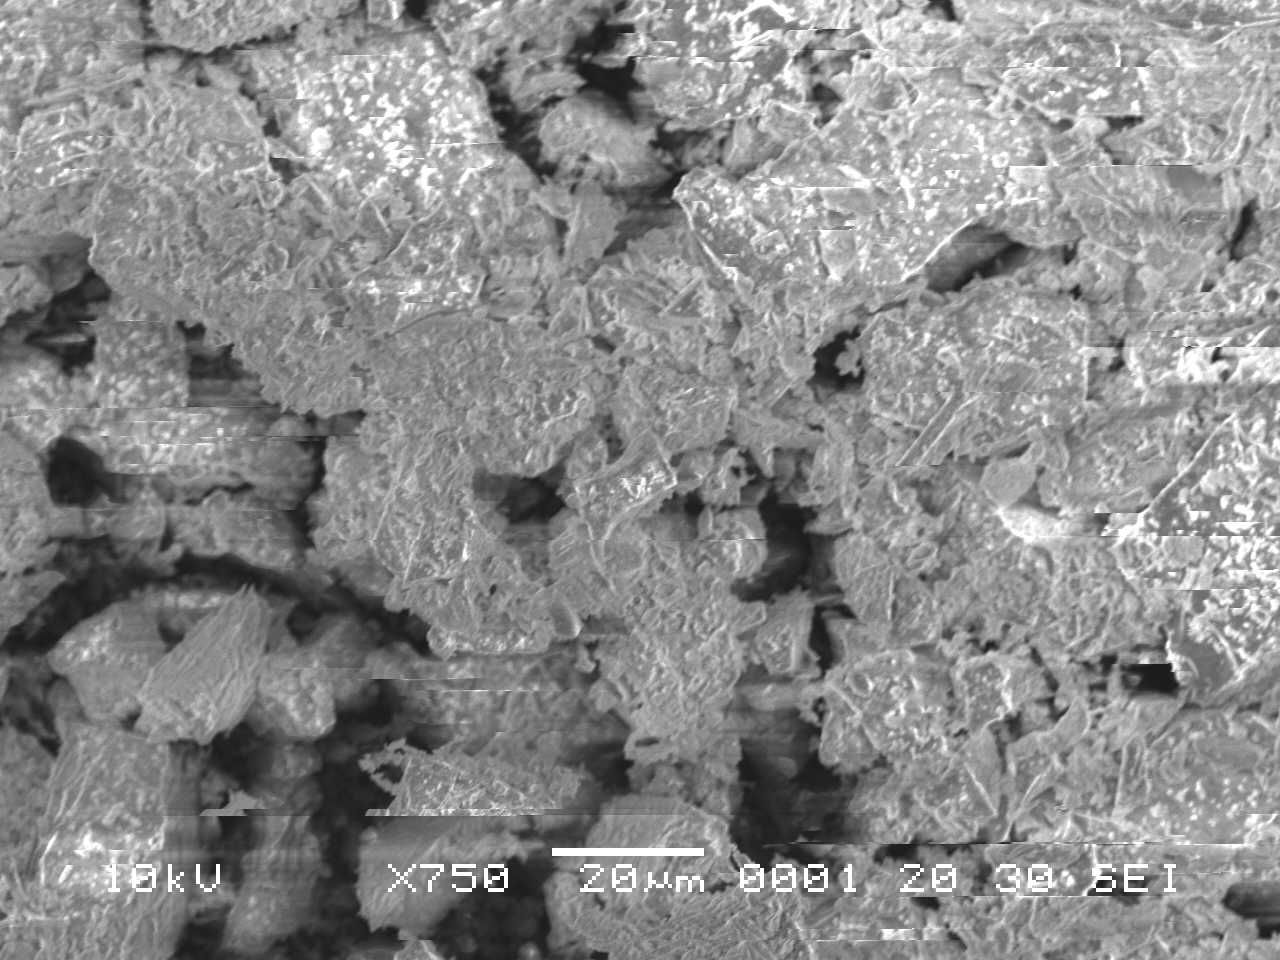
\includegraphics[width=\linewidth]{Az1_x750_3_220221}
\end{minipage}
\begin{minipage}{.45\textwidth}
  \centering
  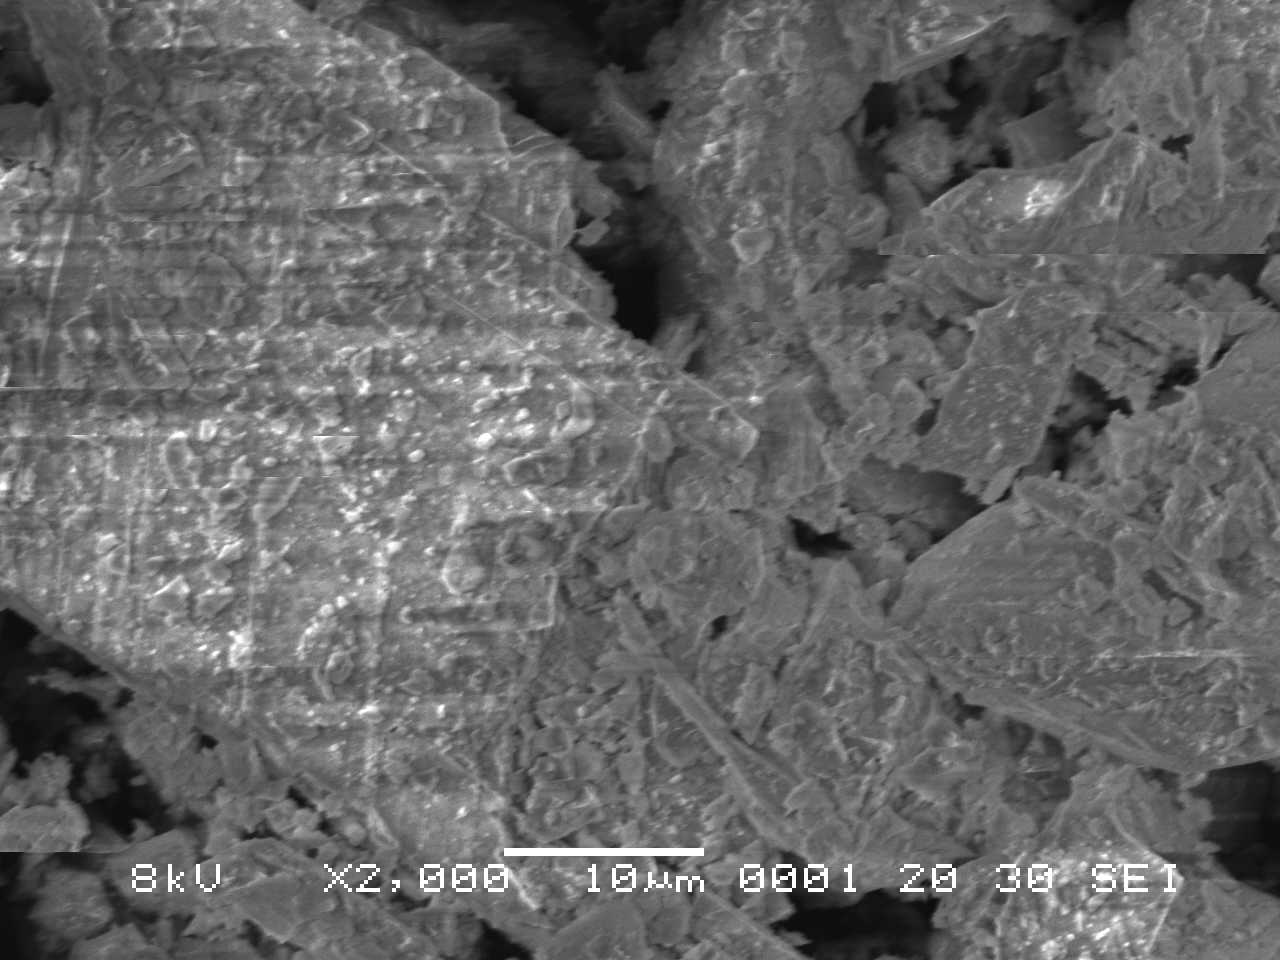
\includegraphics[width=\linewidth]{Az1_x2000_4_220221}
\end{minipage}
\caption[SEM images: Sample Az1, azurite]{SEM images: Sample Az1, azurite. Magnification: \textbf{left)} 750x, \textbf{right)} 2000x.}
\label{fig:az1_sem_1}
\end{figure}


% ************************************************     Az2     *******************************************************************

\textit{Figure \ref{fig:az2_sem_1}} shows sample Az2, which is morphologically significantly different from all other observed samples and lacks the features that appear to correlate with either natural or artificial pigment sources. Surface charging made it difficult to image this sample, and this issue was also not observed with most other samples.

In \textit{Figure \ref{fig:az2_sem_1}}, images of the sample at 200x and 1500x magnifications are shown. It is interesting that although the shape of each sample is quite asymmetric and angular, the size and irregular shape is quite consistent between particules. At 200x magnification, the surface of the particles appears flat and smooth. It is also significant that these particles are much larger than the average particle size observed in other samples, which may suggest industrial pigment grinding. Otherwise, this consistency could also reflect a synthetic origin, with controlled conditions of crystal growth.

At 1500x magnification, there is very little surface texture observed. Sample Az2 is obviously unlike the sample HKI natural azurite. However, it also does not resemble known synthetic samples either. Imaging at higher magnifications was not possible due to charging.

\begin{figure}[H]
\centering
\begin{minipage}{.45\textwidth}
  \centering
  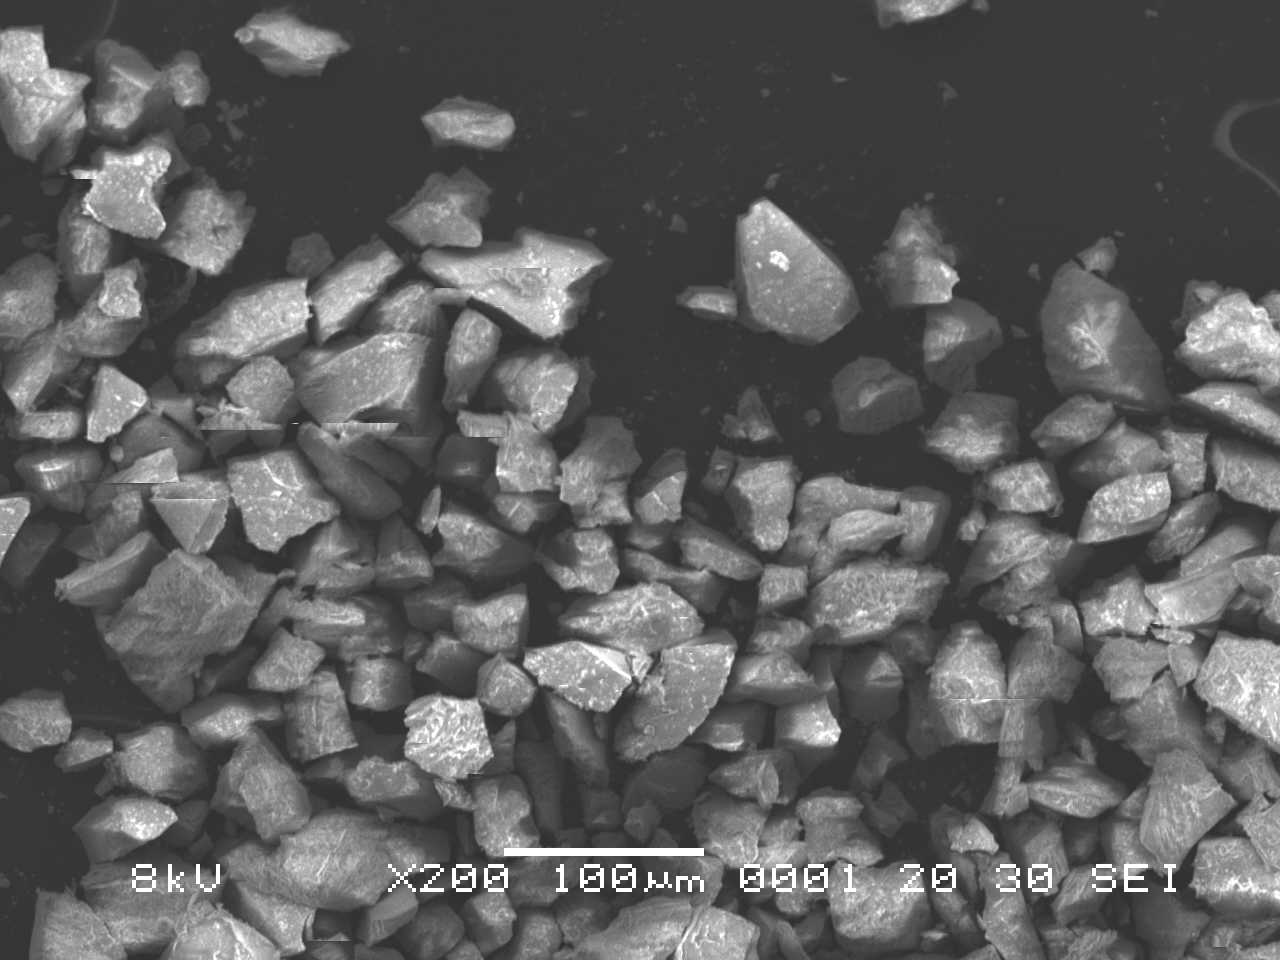
\includegraphics[width=\linewidth]{Az2_x200_1_240221}
\end{minipage}
\begin{minipage}{.45\textwidth}
  \centering
  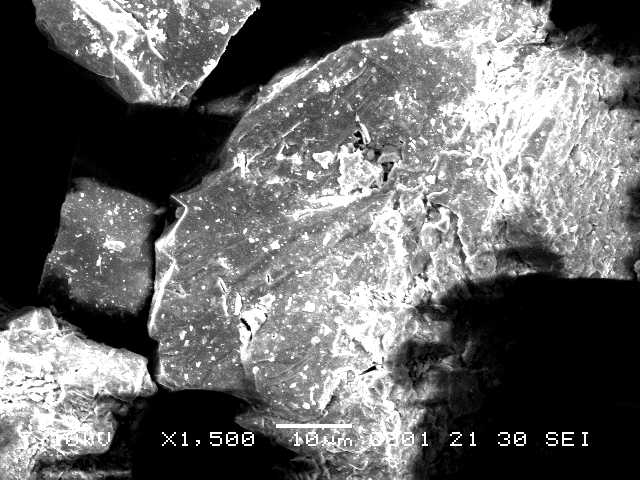
\includegraphics[width=\linewidth]{Az2_x1500_1_150321}
\end{minipage}
\caption[SEM images: Sample Az2, azurite]{SEM images: Sample Az2, azurite. Magnification: \textbf{left)} 200x, \textbf{right)} 1500x.}
\label{fig:az2_sem_1}
\end{figure}


% ************************************************     AzMag     *******************************************************************

\textit{Figure \ref{fig:azmag_sem_1}} show sample AzMag at 750x and 3000x magnifications. At 750x, the surfaces of particles are choppy, rough, and highly textured. Most particles are approximately square or triangular, with a few small spheres on the surface. Elongated and large particles are not observed. At high magnification (3000x), the surface texture of the sample is clearly visualized. The directionality observed in HKI natural azurite at high magnifications is not observed here. However, the degree of roughness and character of the surfaces is very similar, implying that this sample is naturally produced.

\begin{figure}[H]
\centering
\begin{minipage}{.45\textwidth}
  \centering
  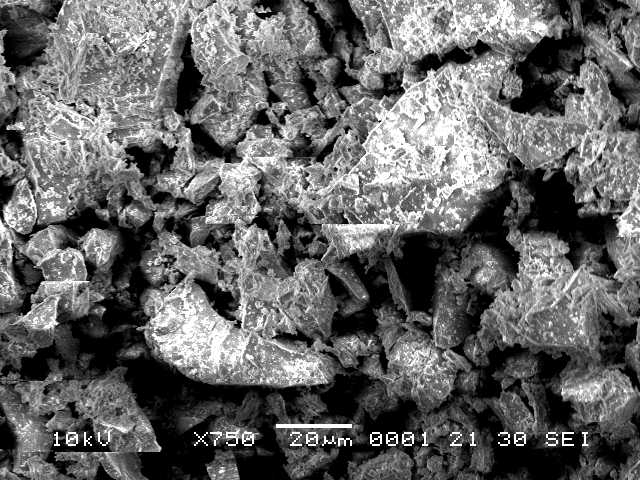
\includegraphics[width=\linewidth]{AzMag_x750_1_160321}
\end{minipage}
\begin{minipage}{.45\textwidth}
  \centering
  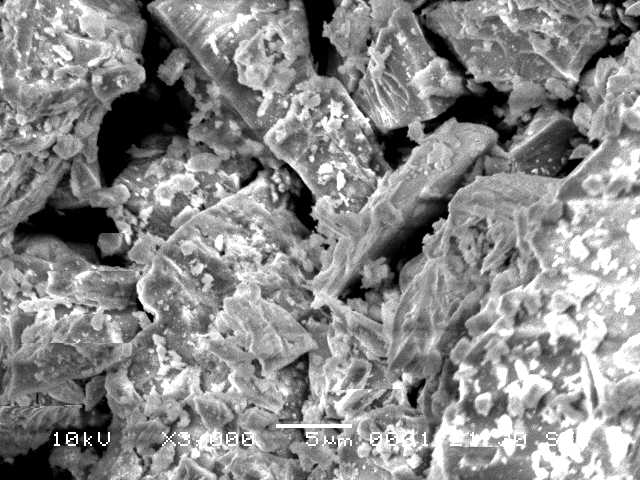
\includegraphics[width=\linewidth]{AzMag_x3000_1_160321}
\end{minipage}
\caption[SEM images: Sample AzMag, azurite]{SEM images: Sample AzMag, azurite. Magnification: \textbf{left)} 750x, \textbf{right)} 3000x.}
\label{fig:azmag_sem_1}
\end{figure}




% ************************************************     AzOp     *******************************************************************

\textit{Figures \ref{fig:azop_sem_1}} and \textit{\ref{fig:azop_sem_2}} show sample AzOp at 750x and 2000x magnifications. 

At 750x magnification (\textit{Figure \ref{fig:azop_sem_1}}, right), it is clear that there are larger particles/aggregations present. It is difficult to tell whether these are in fact single pieces or clumps of smaller particles. The shape of all particles is extremely asymmetrical and varied, except in one specific case; at the bottom of the image there is a cluster of fairly uniformly spherical particles. 

\begin{figure}[H]
\centering
  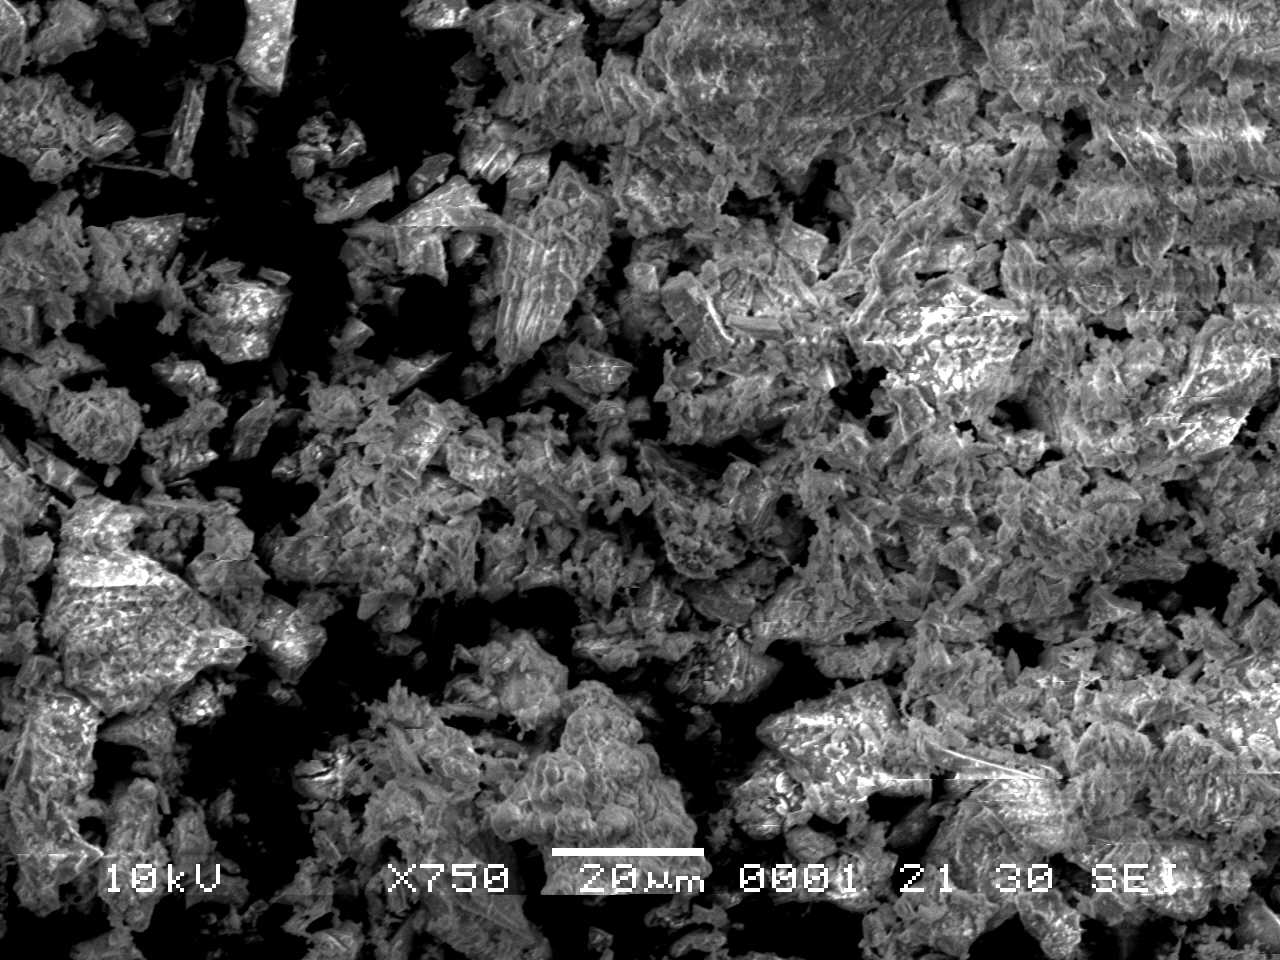
\includegraphics[width=.45\linewidth]{AzOp_x750_2_150321}
\caption[SEM image: Sample AzOp, azurite]{SEM image: Sample AzOp, azurite. Magnification: 750x.}
\label{fig:azop_sem_1}
\end{figure}

The spherical particles are clearly observed in \textit{Figure \ref{fig:azop_sem_2}}, right. They appear bubbly, as if many partial spheres have formed one on top of the other. This texture is not observed extensively in this sample, nor in other samples such as AzMag and HKI natural azurite that are otherwise similar to the rest of sample AzOp. This could be the result of sample contamination, as several samples were analyzed at the same time, or this could be evidence of multiple conditions under which crystals formed before being mixed to make this pigment. Regardless, this type of morphology is quite uniform and does not look like the result of random crushing and grinding. This certainly must be investigated further by imaging over a larger area of this sample as well as by preparing additional fresh samples.

In contrast, the rougher and more heterogenous texture of the majority of the sample is shown at 2000x magnification in \textit{Figure \ref{fig:azop_sem_2}}, left. aVery few remotely circular particles are seen, and there is a great deal of heterogeneity in size and shape. This is very similar to natural samples discussed above.

\begin{figure}[H]
\centering
\begin{minipage}{.45\textwidth}
  \centering
  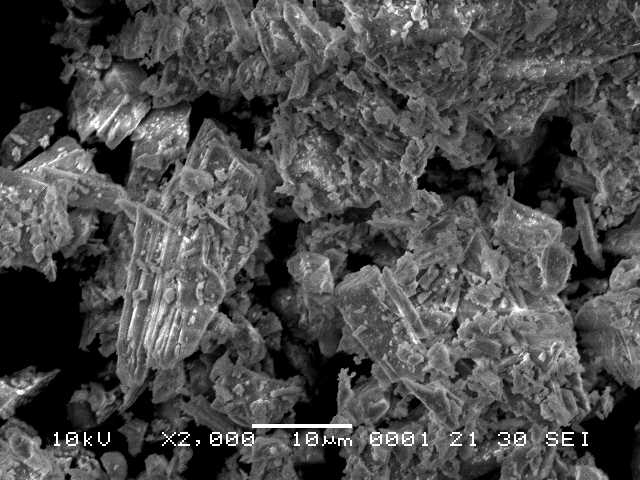
\includegraphics[width=\linewidth]{AzOp_x2000_1_150321}
\end{minipage}
\begin{minipage}{.45\textwidth}
  \centering
  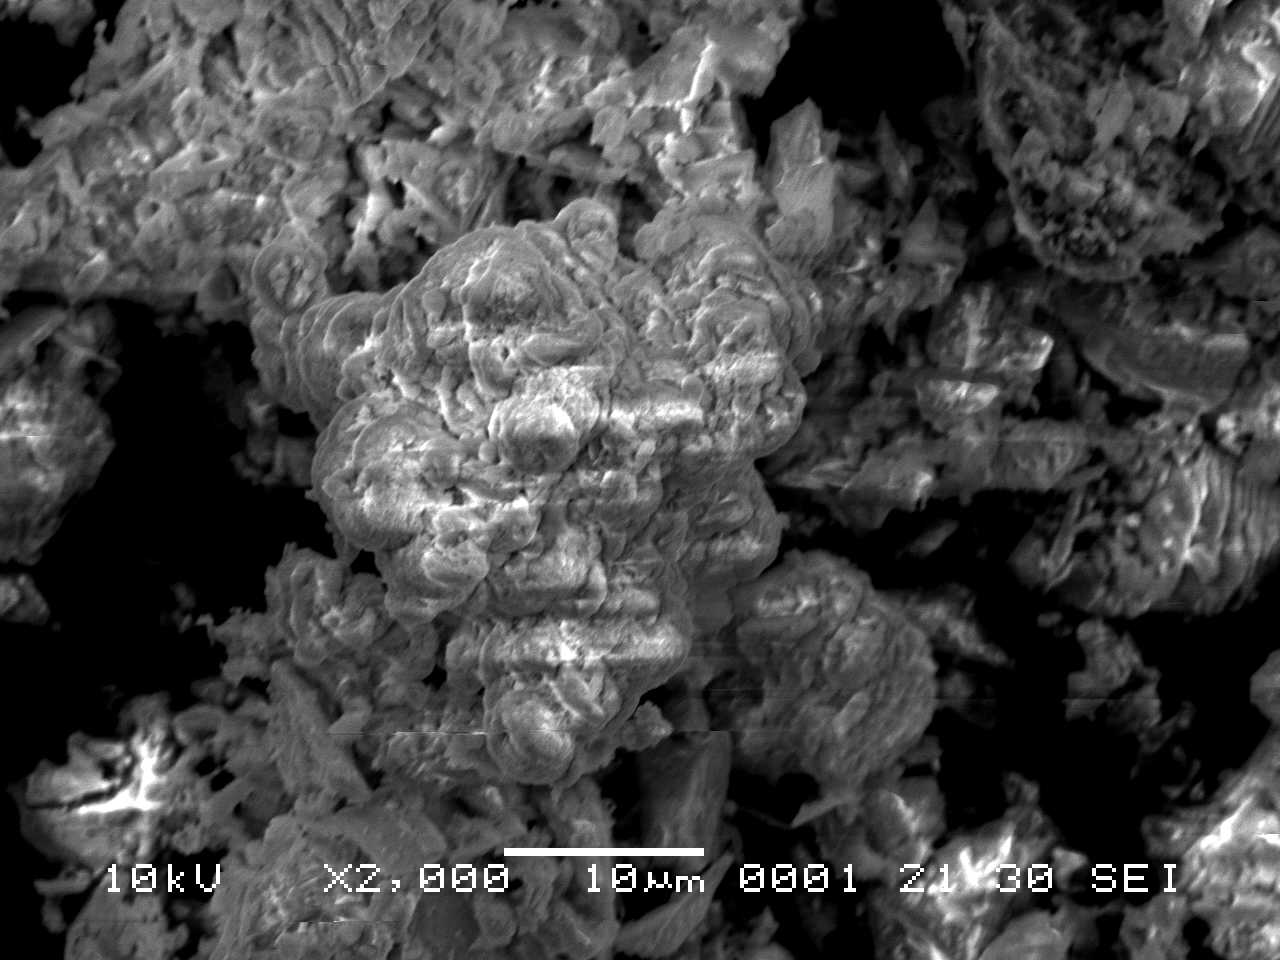
\includegraphics[width=\linewidth]{AzOp_x2000_4_150321}
\end{minipage}
\caption[SEM images: Sample AzOp, azurite]{SEM images: Sample AzOp, azurite. Magnification: 2000x}
\label{fig:azop_sem_2}
\end{figure}

% ************************************************     Fitz1     *******************************************************************
\textit{Figure \ref{fig:Fitz1_sem_1}} shows sample Fitz 1 at 750x and 1500x magnifications. This sample is described as blue verditer, and a commercial product number is provided allowing confirmation that this is a synthetic product.

At 750x magnification (\textit{Figure \ref{fig:Fitz1_sem_1}}, left), it is possible to qualitatively assess the diameter of particles as consistently < 5 $\mu$m. Particles resemble the spherical cluster observed in the sample AzOp. There is regularity of both size and shape, but it is difficult to determine whether the particles are flat discs or stacked semicircles occupying more volume.

At 1500x magnification (\textit{Figure \ref{fig:Fitz1_sem_1}}, right), there are clearly spherical particles. These have formed aggregates, though it is not clear whether individual particles could be separated back out of the larger clusters. The size is similar to the spherical cluster in the AzOp sample. The surface also looks slightly pocked or porous. 

\begin{figure}[H]
\centering
\begin{minipage}{.45\textwidth}
  \centering
  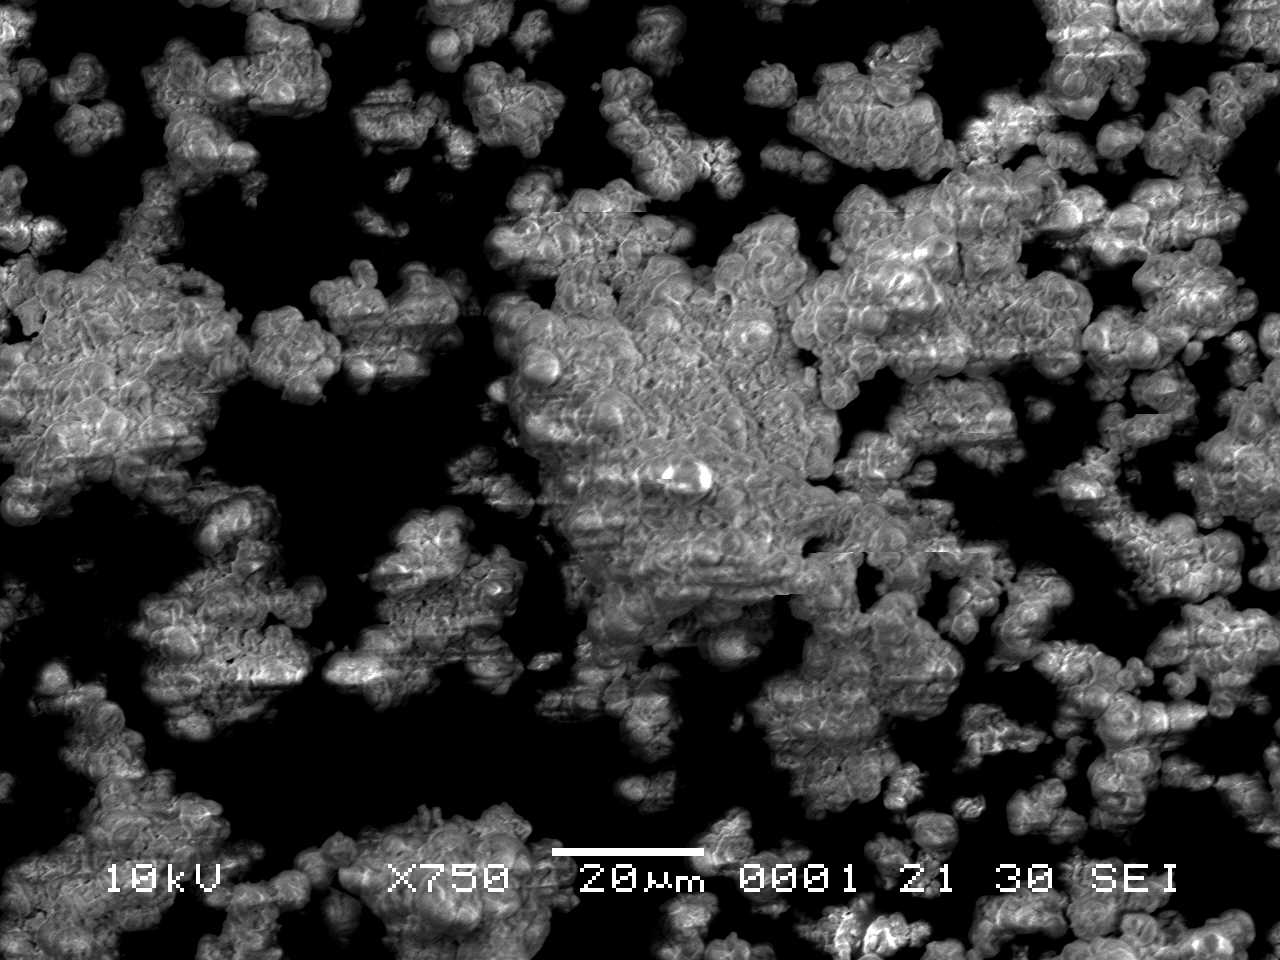
\includegraphics[width=\linewidth]{Fitz1_x750_1_030321}
\end{minipage}
\begin{minipage}{.45\textwidth}
  \centering
  \includegraphics[width=\linewidth]{Fitz1_x1500_2_030321}
\end{minipage}
\caption[SEM images: Sample Fitz1, blue verditer]{SEM images: Sample Fitz1, blue verditer. Magnification: \textbf{left)} 750x, \textbf{right)} 1500x}
\label{fig:Fitz1_sem_1}
\end{figure}


% ************************************************     KE3     *******************************************************************

\textit{Figure \ref{fig:KE3_sem_1}} shows sample KE 3 at 750x and 2000x magnifications. The sample is described as light verditer bice. Verditer suggests a synthetic origin, while bice is used to refer to both natural and synthetic blue pigments. Tentatively, this sample is interpreted to be synthetic based on this information.

At 750x magnification (\textit{Figure \ref{fig:KE3_sem_1}}, left), the uniformity of the particles is apparent. They are fairly symmetric and spherical, but more angular than sample Fitz1. There are some areas of needle-like structures as well as stacks of spherical or octagonal particles forming small aggregates. At 2000x magnification (\textit{Figure \ref{fig:KE3_sem_1}}, right), spheres are observed. There is significant texture on the surface that is quite fine especially around the edges of particles, and this texture appears rougher than that of sample Fitz 1. This may be due, though, to poorer image quality of the Fitz 1 sample. The approximate particle size can be approximated to 5-10 $\mu$m.

\begin{figure}[H]
\centering
\begin{minipage}{.45\textwidth}
  \centering
  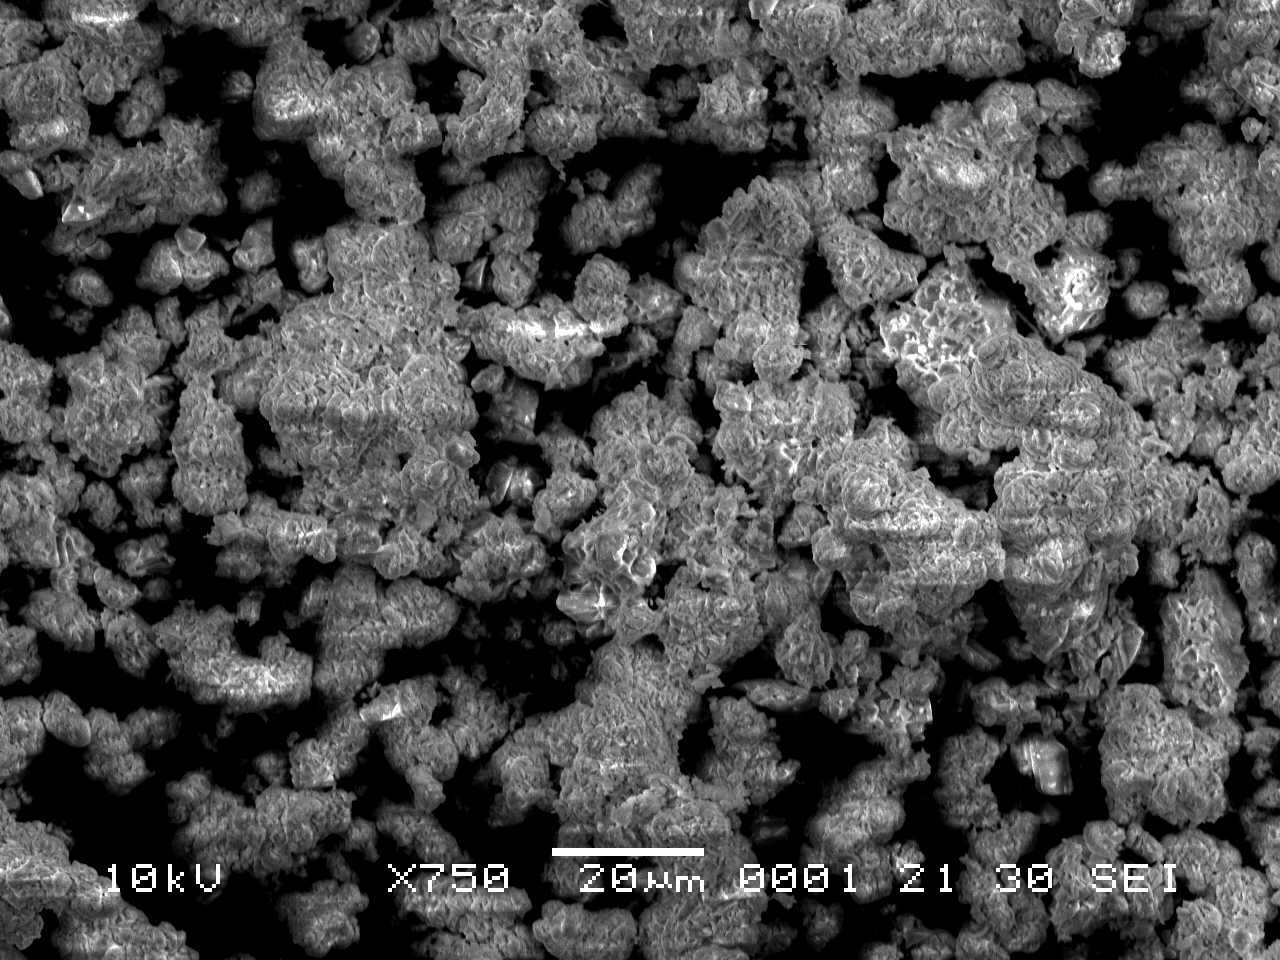
\includegraphics[width=\linewidth]{KE3_x750_3_050321}
\end{minipage}
\begin{minipage}{.45\textwidth}
  \centering
  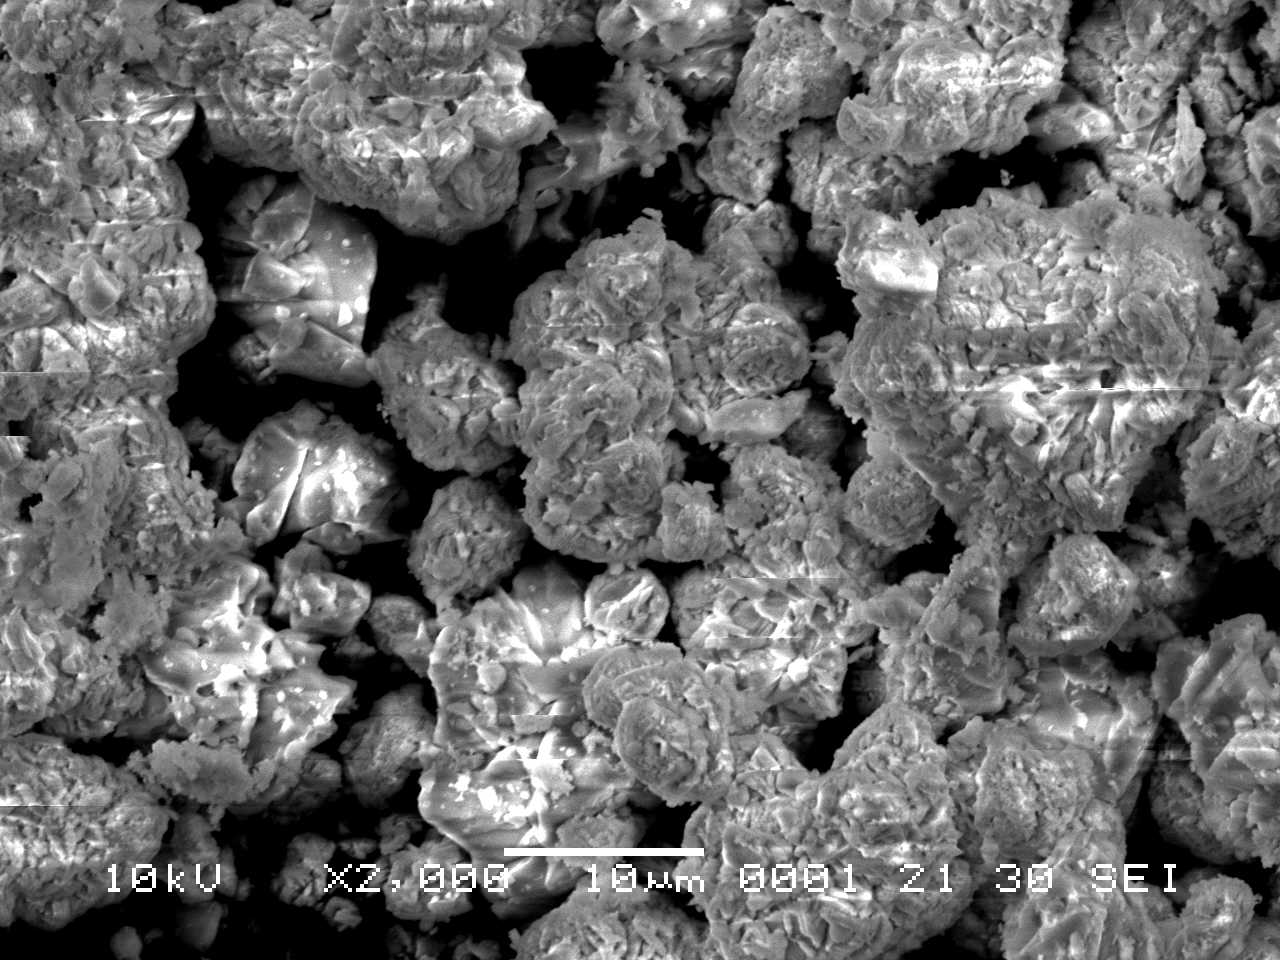
\includegraphics[width=\linewidth]{KE3_x2000_2_050321}
\end{minipage}
\caption[SEM images: Sample KE3, light verditer bice]{SEM images: Sample KE3, light verditer bice. Magnification: \textbf{left)} 750x, \textbf{right)} 2000x}
\label{fig:KE3_sem_1}
\end{figure}

% ************************************************     KE4     *******************************************************************

\textit{Figure \ref{fig:KE4_sem_1}} shows sample KE 4 at magnifications at 750x and 2000x. KE 4 is labelled as blue bice, which is an ambiguous description, so it is inconclusive whether this sample was prepared naturally or synthetically.

At 750x magnification (\textit{Figure \ref{fig:KE4_sem_1}}, left), fine needle-like structure is visible similar to that of sample HKI natural azurite. At the same time, there are also rounder structures that resemble Fitz 1. Larger particles on the order of 50 $\mu$m are visible, as are significantly smaller particles on the order of 5 $\mu$m. \textit{Figure \ref{fig:KE4_sem_1}} (right) shows KE 4 at 2000x magnification. The image is focused on the flat side of a larger particle (or aggregate) with many smaller particles attached to or resting on the surface. There are also pockmarks or cavities observed. This sample is ambiguous as it shows characteristics of known natural as well as synthetic samples.

\begin{figure}[H]
\centering
\begin{minipage}{.45\textwidth}
  \centering
  \includegraphics[width=\linewidth]{KE4_x750_1_030321}
\end{minipage}
\begin{minipage}{.45\textwidth}
  \centering
  \includegraphics[width=\linewidth]{KE4_x2000_1_030321}
\end{minipage}
\caption[SEM images: Sample KE4, blue bice]{SEM images: Sample KE4, blue bice. Magnification: \textbf{left)} 750x, \textbf{right)} 2000x}
\label{fig:KE4_sem_1}
\end{figure}


% ************************************************     KE5     *******************************************************************

\textit{Figure \ref{fig:KE5_sem_1}} shows sample KE 5 at 750x and 1500x magnifications. KE 5 is described as blue verditer, strongly suggesting a synthetic origin.

\textit{Figure \ref{fig:KE5_sem_1}} (left) shows KE 5 at 750x magnification. At this magnification, larger aggregates of approximately 80 $\mu$m are clearly seen to be formed from smaller particles. This is very similar to the appearance of Fitz 1 at the same magnification. The appearance also brings to mind the crystal formation of desert rose gypsum, characterized by intersecting flat discs forming circular or semicircular three dimensional structures. \textit{Figure \ref{fig:KE5_sem_1}} (right) shows KE 5 at 1500x magnification. The circular character of particles is very clearly observed in these images.

%~\autocite{hope_gypsum}

\begin{figure}[H]
\centering
\begin{minipage}{.45\textwidth}
  \centering
  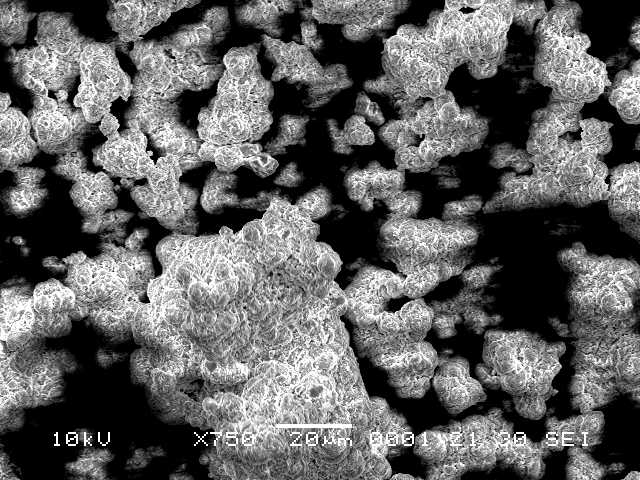
\includegraphics[width=\linewidth]{KE5_x750_1_050321}
\end{minipage}
\begin{minipage}{.45\textwidth}
  \centering
  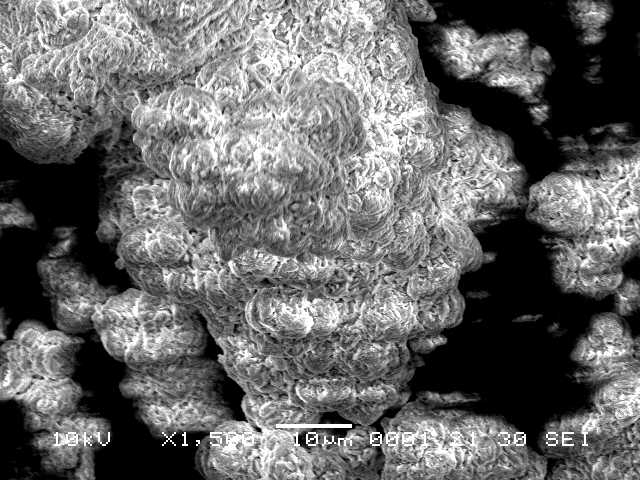
\includegraphics[width=\linewidth]{KE5_x1500_1_050321}
\end{minipage}
\caption[SEM images: Sample KE 5, blue verditer]{SEM images: Sample KE 5, blue verditer. Magnification: \textbf{left)} 750x, \textbf{right)} 1500x}
\label{fig:KE5_sem_1}
\end{figure}

\subsubsection[Particle size distribution of natural and artificial azurite]{Particle size distribution of natural and artificial azurite}
\label{subsubsection3.1.1.1}

SEM images at 750x magnification were collected from edges of loose pigments samples used for SEM analysis above where particles were most loosely dispersed. The two powder samples selected, HKI natural azurite and Fitz 1, were selected on the basis of their known sources as well as significantly different morphology. The historical cross section was also analysed using the same method. These images were processed in ImageJ (Version 1.53a) by increasing contrast and manually thresholding followed by manual selection of maximum lengths and measurement using the image scale bar. 

Five images of Fitz 1 were analysed, with n(particles) = 102. Five images of HKI natural azurite were analysed, with n(particles) = 127. Three images of the historical cross section were analysed, with n(particles) = 153. There is undoubtedly some bias in selected particles due to the difficulty of defining edges in the images, and this may affect the spread of results. An example of the original SEM image (left) and the thresholded binary image (right, used for measurements) is shown for sample Fitz 1 in \textit{Figure \ref{fig:imageJ_fitz1}}.

\begin{figure}[H]
\centering
\begin{minipage}{.45\textwidth}
  \centering
  \includegraphics[width=\linewidth]{Fitz1_x750_5_130521}
\end{minipage}
\begin{minipage}{.45\textwidth}
  \centering
  \includegraphics[width=\linewidth]{Fitz1_x750_5_130521_BW}
\end{minipage}
\caption[Particle size analysis: Sample Fitz 1]{Particle size analysis: Sample Fitz 1. \textbf{Left)} original SEM image, \textbf{Right)} thresholded binary image.}
\label{fig:imageJ_fitz1}
\end{figure}

The measurements from each sample image were combined and analysed using R (RStudio Version 1.3.1093) to produce a histogram of the frequency of length measurements (bin size = 1 $\mu$m) for each sample, shown in \textit{Figure \ref{fig:histogram_length}}. Based on the different particle morphologies, it would be reasonable to expect that the particle size distribution would differ between samples. Additionally, the presence of a bimodal distribution in the histogram might indicate the formation of aggregates of a specific size from single particles. 

The length distributions of Fitz 1 and HKI natural azurite do not show significant differences. Both show a high frequency of particles with lengths around 5 $\mu$m, with a low frequency of particles or clusters above 10 $\mu$m. Sample Fitz 1 does appear to have several particles of length around 15 $\mu$m, which is absent in HKI natural azurite. This could suggest that aggregates are forming at more consistent sizes than in sample HKI natural azurite. Overall, though, these two samples are statistically very similar in this analysis. \textit{Table \ref{table:r_stats}} contains descriptive statistics, and it is notable how similar the means (and to some extent medians) are between all three samples. There is a notably larger range of particle lengths in the natural azurite sample, though this may be an artifact of processing since the historical cross section shows overall smaller particle sizes than both powder samples. 

\begin{figure}[H]
\centering
\begin{minipage}{.45\textwidth}
  \centering
  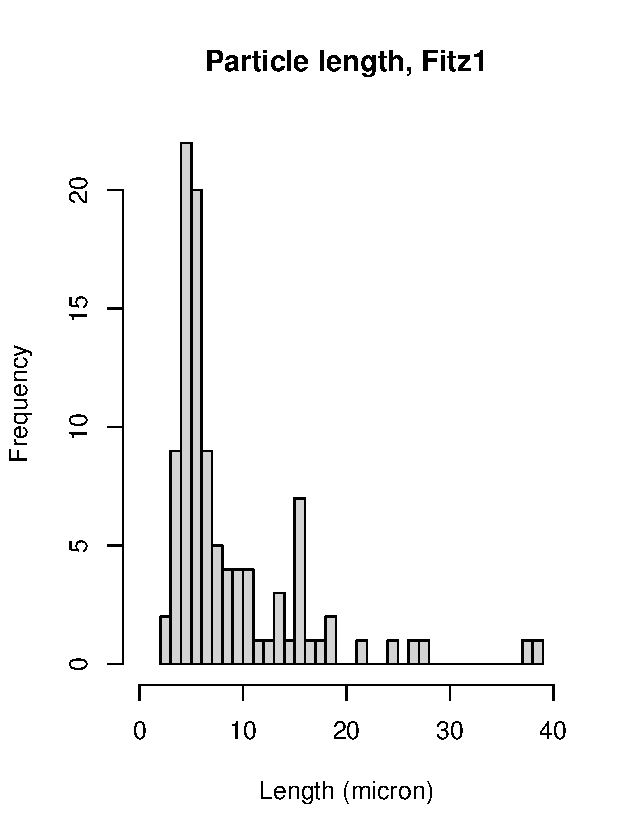
\includegraphics[width=\linewidth]{hist_fitz1}
\end{minipage}
\begin{minipage}{.45\textwidth}
  \centering
  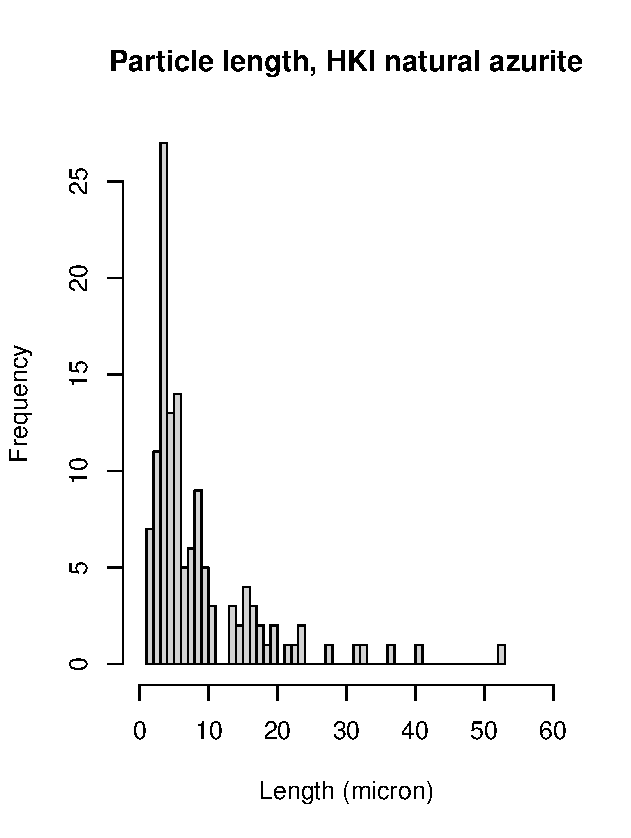
\includegraphics[width=\linewidth]{hist_hki}
\end{minipage}
\caption[Particle size analysis: HKI natural azurite, Fitz 1]{Particle size analysis: Sample HKI natural azurite. \textbf{Left)} Fitz 1, \textbf{Right)} HKI natural azurite.}
\label{fig:histogram_length}
\end{figure}

\begin{figure}[H]
\centering
  \includegraphics[width=0.45\linewidth]{hist_xsection}
\caption[Particle size analysis: historical cross section]{Particle size analysis: historical cross section.} 
\label{fig:hist_xsec}
\end{figure}

\begin{table}[H]
\caption{Descriptive statistics: Fitz 1, HKI natural azurite, historical cross section}
\centering
\label{table:r_stats}
\begin{tabular}{c c c c}
\toprule
Reference sample & Mean & Median & Range \\
\midrule
HKI natural azurite & 8.583 & 5.437 & 1.177 - 52.176 \\
Fitz 1 & 8.683 & 5.878 & 2.414 - 38.367 \\
Historical cross section & 8.328 & 7.648 & 2.142 - 28.930 \\
\bottomrule
\end{tabular}
\end{table}

Lengths of the three samples are compared side-by-side in \textit{Figure \ref{fig:hist_all}}. The effect of outliers on the mean values of particle sizes is apparent, since both powder samples (black, red) show length distributions that, apart from a few larger outliers, are located at smaller lengths than that of the cross section in spite of all three datasets having very similar mean values. 

The difference between the powder samples and the cross section may be due to a number of factors. The preparation of pigments likely differed in the 15th century as compared to today, though azurite's optical properties depend on the size of its particle grains and we may therefore expect the fineness of grinding not to vary wildly. 

The suspension in a binding medium would be expected to affect the dispersion of grains, and this could reasonably affect aggregation (whether or not it would hinder aggregation depends on the hydrophilicity of the mineral, which is low in the case of azurite).~\autocite{Zhang} Optimal dispersion may also be orientation dependent. As discussed above, sampling bias will be present as only the x and y dimensions of the grains can be measured using this method, and depending on the orientation of particles relative to the slicing of the cross section, certain orientations may be over or underrepresented. 

The preparation of the cross section by resin embedding followed by microtoning will affect the appearance of particles under SEM. Microtoning may visually flatten the particles, making it difficult to see smaller grains. 

\begin{figure}[H]
\centering
  \includegraphics[width=0.9\linewidth]{hist_fitz1_hki_xsec_largerange}
\caption[Particle size analysis: HKI natural azurite, Fitz 1, historical cross section]{Particle size analysis: Fitz 1 (black), HKI natural azurite (red), historical cross section (blue).} 
\label{fig:hist_all}
\end{figure}


%fitz 1
%Median : 5.878  
%Mean   : 8.683
%range 2.414 to 38.367
% hki 
%Median : 5.437  
%Mean   : 8.583
%range 1.177 to 52.176

% *******************************************************************************************************************************
% *******************************************************************************************************************************
% *******************************************************************************************************************************

\subsection[Malachite and green verditer]{Malachite and green verditer}
\label{subsection3.1.2}

% ************************************************     Ma1     *******************************************************************

\textit{Figures \ref{fig:Ma1_sem_1}} and \textit{\ref{fig:Ma1_sem_2}} show sample Ma1 at magnifications from 750x to 3000x. This sample is natural malachite.

At 750x magnification (\textit{Figure \ref{fig:Ma1_sem_1}}, left), the particles appear highly irregular. Particles have extremely rough and choppy edges, and these irregular shapes closely resemble those of natural azurite samples in terms of their roughness and sharpness. There are few aggregates or clumps that are larger than 20 $\mu$m.  

\textit{Figure \ref{fig:Ma1_sem_2}} (left) shows the sample at 2500x magnification. It is disordered and heterogeneous. While it is possible that this is due to grinding the pigment during preparation, \textit{Figure \ref{fig:Ma1_sem_2}} (right) shows further disorder at 3000x. Here, many particles under 1 $\mu$m across are present, with extremely uneven borders. These are unambiguously single particles rather than surface roughness on a larger plane.

\begin{figure}[H]
\centering
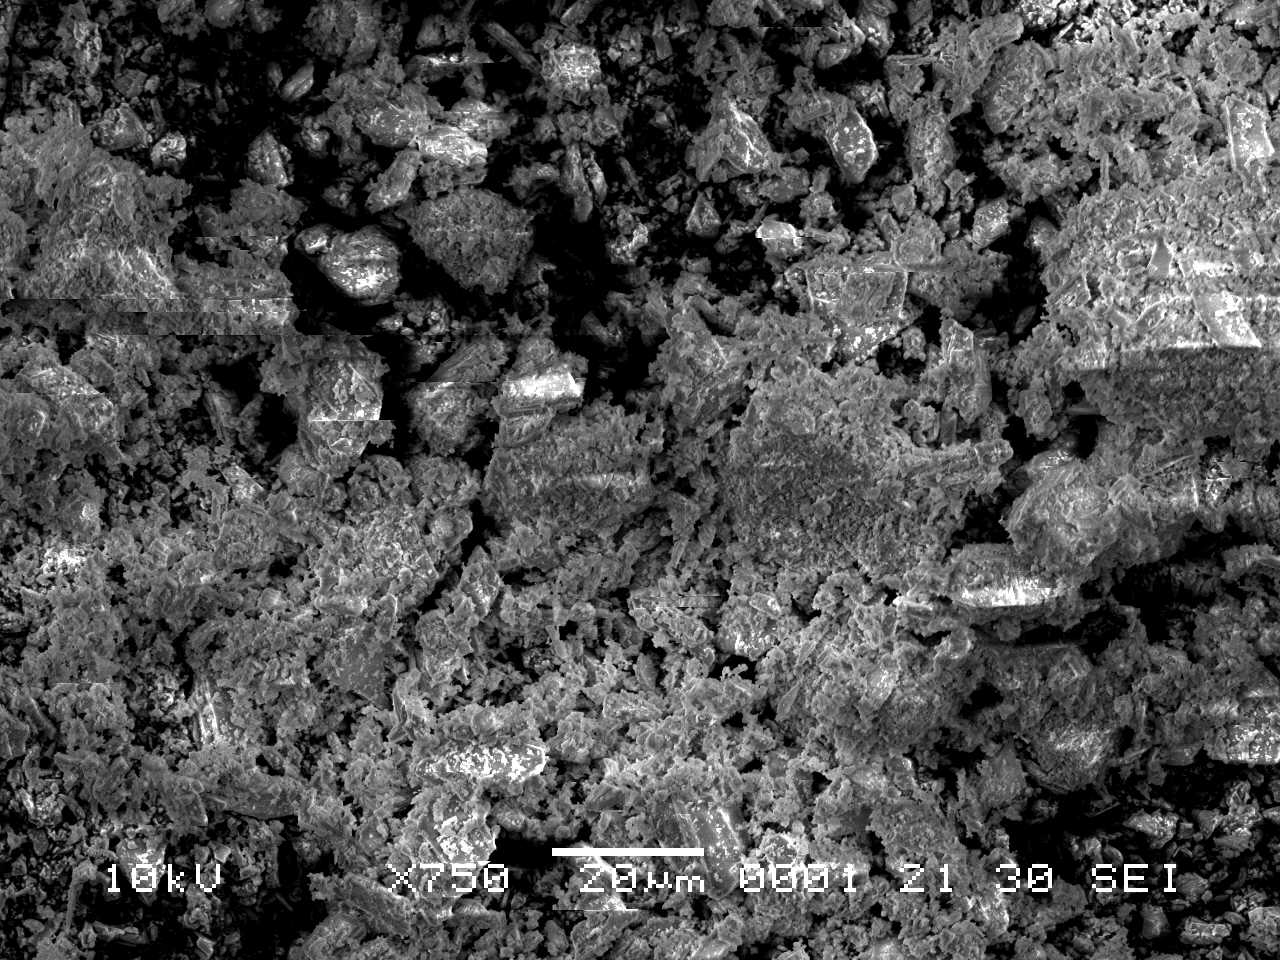
\includegraphics[width=0.45\linewidth]{Ma1_x750_2_160321}
\caption[SEM images: Sample Ma 1, malachite]{SEM images: Sample Ma 1, malachite. Magnification: 750x.}
\label{fig:Ma1_sem_1}
\end{figure}

\begin{figure}[H]
\centering
\begin{minipage}{.45\textwidth}
  \centering
  \includegraphics[width=\linewidth]{Ma1_x2500_3_160321}
\end{minipage}
\begin{minipage}{.45\textwidth}
  \centering
  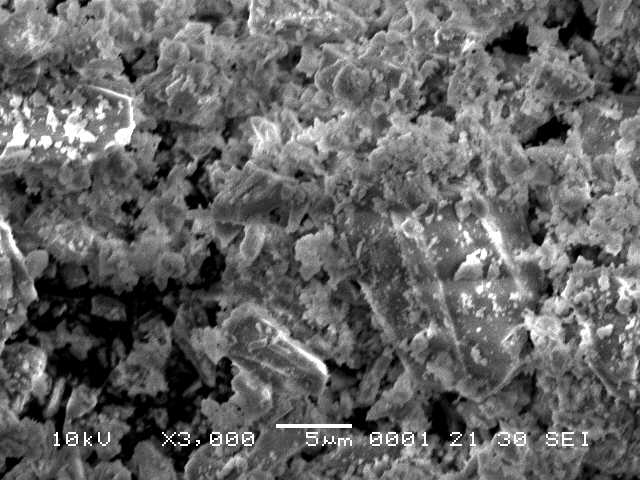
\includegraphics[width=\linewidth]{Ma1_x3000_2_160321}
\end{minipage}
\caption[SEM images: Sample Ma 1, malachite]{SEM images: Sample Ma 1, malachite. Magnification: \textbf{left)} 2500x, \textbf{right)} 3000x.}
\label{fig:Ma1_sem_2}
\end{figure}

% ************************************************     KE1a     *******************************************************************

\textit{Figure \ref{fig:KE1a_sem_1}} shows sample KE 1a at magnifications 250x (left) and 750x (right). The name of KE 1a, green bice, is ambiguous and could refer to a natural or an artificial sample.

At 250x magnification, small particles form aggregations of approximately 25-50 $\mu$m. The image at 750x magnification is poor quality, and charging prevented use of higher magnifications. The shapes of particles do appear to be squared-off circles with some degree of uniformity. They are not, however, spherical like several of the blue pigment samples discussed above. 

This sample is qualitatively more uniform than sample Ma 1, and more spherical, but it is more challenging to draw clear conclusions about morphological differences between natural and synthetic green samples compared to blue. There is a much smaller sample size in the reference samples available, as well as ambiguity in sample source, but this also may just mean that green samples do not show marked morphology changes depending on production process.

\begin{figure}[H]
\centering
\begin{minipage}{.45\textwidth}
  \centering
  \includegraphics[width=\linewidth]{KE1a_x250_1_040321}
\end{minipage}
\begin{minipage}{.45\textwidth}
  \centering
  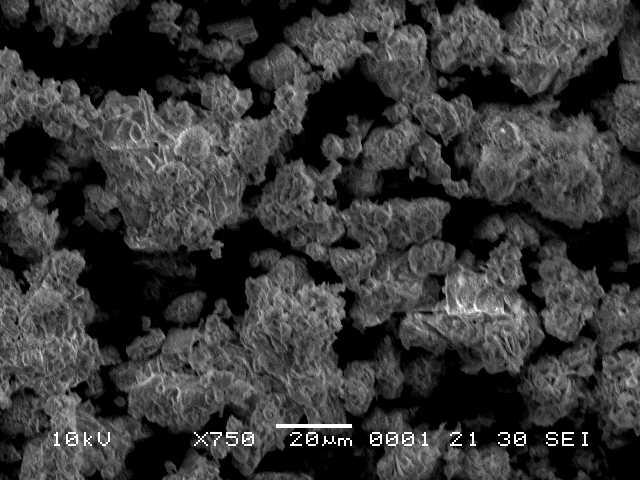
\includegraphics[width=\linewidth]{KE1a_x750_2_040321}
\end{minipage}
\caption[SEM images: Sample KE 1a, green bice]{SEM images: Sample KE 1a, green bice. Magnification: \textbf{left)} 250x, \textbf{right)} 750x}
\label{fig:KE1a_sem_1}
\end{figure}

% ************************************************     KE1b     *******************************************************************

%didnt do this one

% ************************************************     KE2     *******************************************************************

\textit{Figure \ref{fig:KE2_sem_1}} shows sample KE 2, green verditer. The sample name strongly suggests a synthetic source. 

In \textit{Figure \ref{fig:KE2_sem_1}}, the sample is shown at 750x (left) and 2000x (right) magnifications. At 750x magnification (left), particles are very irregularly shaped, sharp, and generally not elongated. At 2000x magnification (right), there is a lack of texture on the surface of individual particles. The edges of particles are extremely feathery, which is observed in other samples discussed in this section as well. It is possible to estimate the particle size at approximately 7-10 $\mu$m. 

\begin{figure}[H]
\centering
\begin{minipage}{.45\textwidth}
  \centering
  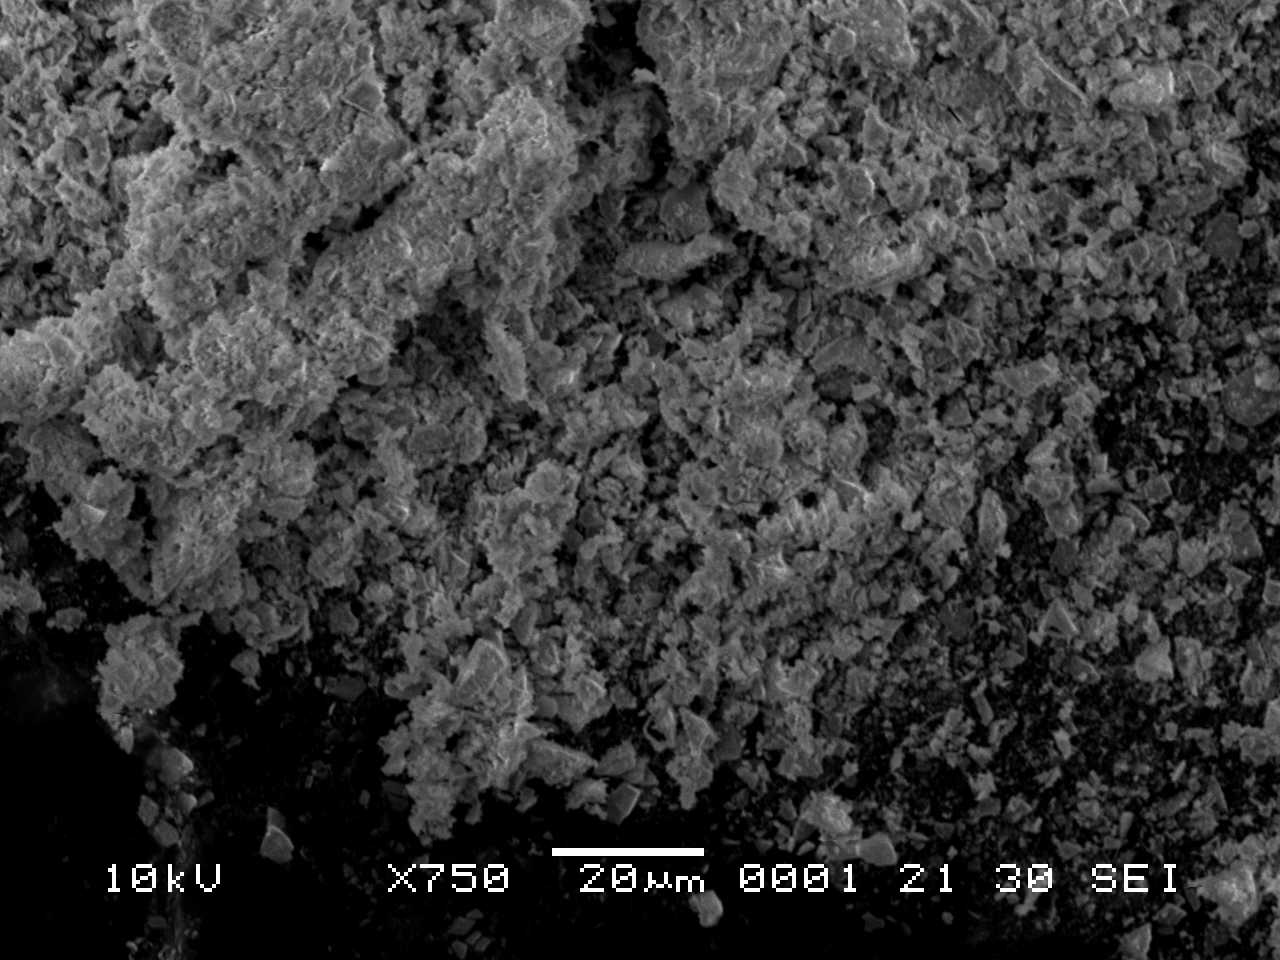
\includegraphics[width=\linewidth]{KE2_x750_1_040321}
\end{minipage}
\begin{minipage}{.45\textwidth}
  \centering
  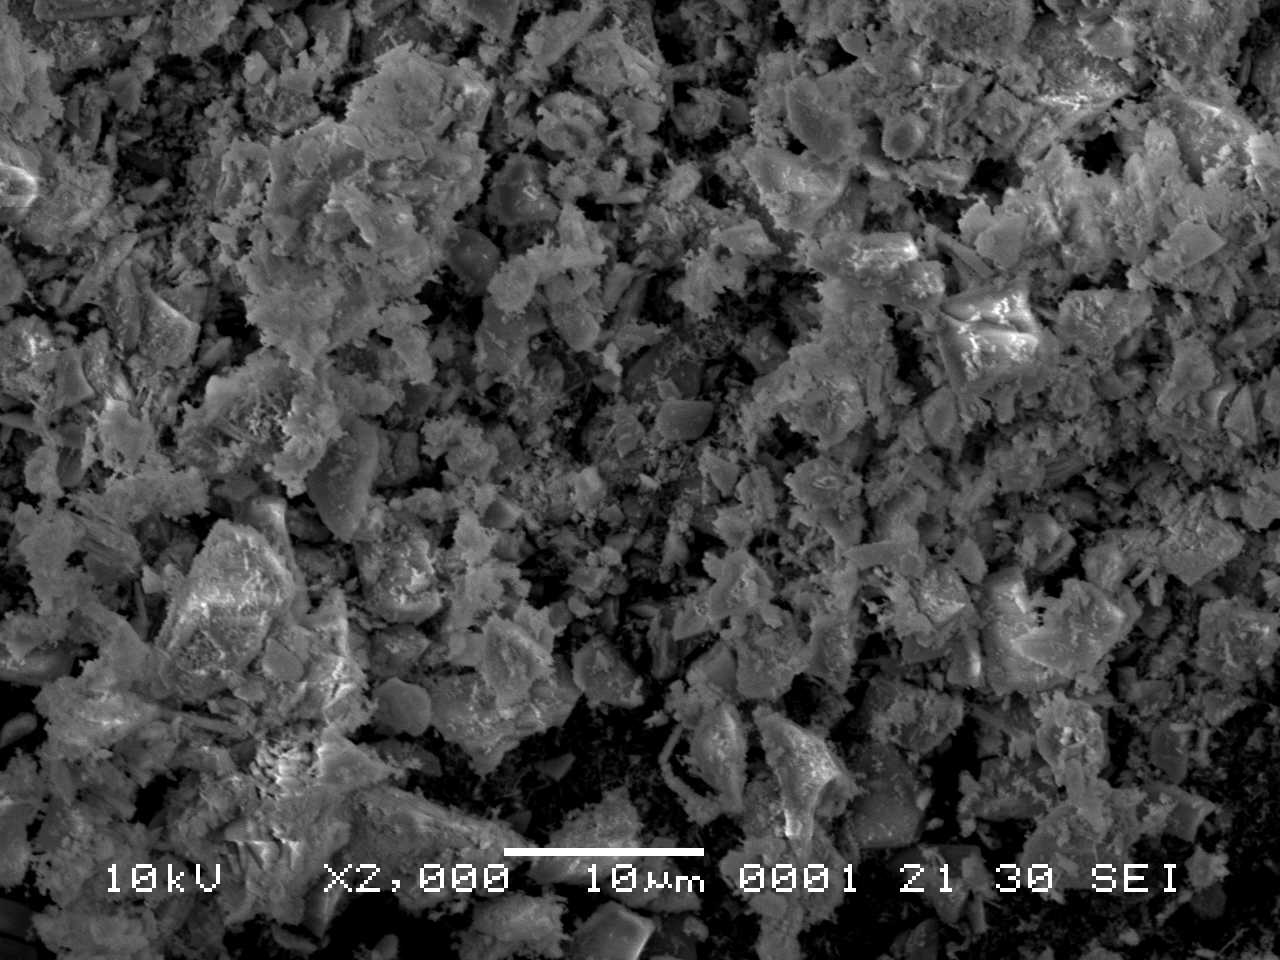
\includegraphics[width=\linewidth]{Ke2_x2000_1_040321}
\end{minipage}
\caption[SEM images: Sample KE2, green verditer]{SEM images: Sample KE2, green verditer. Magnification: \textbf{left)} 750x, \textbf{right)} 2000x}
\label{fig:KE2_sem_1}
\end{figure}


\subsection[Historical samples]{Historical samples}
\label{subsection3.1.3}

SEM images of a historical cross section removed from a 16th c. old masters work (\textit{Birth of Jupiter}, Giulio Romano, azurite/verditer layers c. 1530 and 1630) are presented.

Images were collected on two different instruments, a JEOL JSM-5510LV SEM (coupled with an Oxford Instruments INCA EDS system) and a TESCAN MIRA3 FEG-SEM (coupled with an Oxford Instruments Aztec Energy X-maxN 80 EDS system). The sample was coated with 24 nm carbon to decrease charging. On the JEOl SEM, images were collected using the backscatter electron detector (BES) which is sensitive to the atomic weight of the elements present in the sample: heavier elements will appear lighter in BES images. The BES detector was used in low vacuum mode to prevent sample charging. On the TESCAN SEM, images were collected using the secondary electron detector (SE) and the BES detector simultaneously. 

\textit{Figure \ref{fig:xsection_jeol_1}} (left) shows the cross section at low magnification (750x) collected on the JEOl instrument. The entire width of the cross section is shown, and three distinct layers are visible. The sample contains natural azurite and artificial blue verditer pigment particles, as well as other pigments that are not copper based and, presumably, some form of organic binder in which the pigment particles are embedded. Thin cracks can be seen dividing the pigment layers as well as through the entire cross section vertically. \textit{Figure \ref{fig:hki_crossec_explanation}} labels these three layers A, B, C, with C containing, per the intensity of the BES image, relatively lower atomic weight components. 

The size and shape of pigment particles is extremely uneven. The medium grey pigment in layers A and B is copper based according to EDX results (discussed in next section). EDX results also allow assignment of the bright white particles and aggregates to lead, likely a lead carbonate based on the presence of oxygen and absence of chromium (a component of lead yellow) as well as the color of the cross section under magnification. The copper based particles are morphologically distinct from the lead and manganese (darkest) particles, with dimensions on the order of 10-20 $\mu$m. Discussion of the copper containing pigments follows.

\textit{Figures \ref{fig:xsection_jeol_1}} (right) and \textit{\ref{fig:xsection_jeol_2}} show the cross section at high magnification (1400-2500x) using the JEOL instrument, and \textit{Figures \ref{fig:xsection_dept_1}} and \textit{\ref{fig:xsection_dept_2}} show the cross section at 4300x and 12,500x magnification using the TESCAN instrument. The JEOl instrument in BES shows much more apparent contrast between different elements than the TESCAN instrument, and this makes it slightly more straightforward to interpret. The TESCAN instrument, on the other hand, shows both BES (left) and SE (right) images and offers much sharper resolution but allows poor distinguishing between pigments without the use of mapping. These images capture the structure of the bound cross section clearly, with areas of pitting and cracking visible. One feature that is not easily explained is the feathery, indistinctly bound areas of white in the BES images. As this feature is not present in the SE images, it is not explained by surface charging. Morphologically, it looks to be due to an organic layer of binder or embedding resin rather than due to any pigment.

At higher magnification, the irregularity of orientation and shape of particles is clear. \textit{Figure \ref{fig:xsection_dept_2}} shows the sample at high magnification in an area where copper blue pigments are expected to be present. Here, interesting planar morphology is shown which resembles that of samples Az 1 and AzMag.

\begin{figure}[H]
\centering
  \includegraphics[width=0.6\linewidth]{hki_crossec_explanation}
\caption[Historical cross section with visually distinct layers A, B, and C labelled]{Historical cross section, SEM image at 550x magnification, with visually distinct layers A, B, and C labelled.}
\label{fig:hki_crossec_explanation}
\end{figure}

\begin{figure}[H]
\centering
\begin{minipage}{.45\textwidth}
  \centering
  \includegraphics[width=\linewidth]{hki_xsection_BES_LV_x750_2_58spot_240621}     
\end{minipage}
\begin{minipage}{.45\textwidth}
  \centering
  \includegraphics[width=\linewidth]{hki_xsection_BES_LV_x2500_2_40spot_250621}    
\end{minipage}
\caption[SEM images: Historical cross section, azurite and blue verditer]{SEM images: Historical cross section, azurite and blue verditer. Magnification: \textbf{left)} 750x, \textbf{right)} 2500x}
\label{fig:xsection_jeol_1}
\end{figure}

\begin{figure}[H]
\centering
\begin{minipage}{.45\textwidth}
  \centering
  \includegraphics[width=\linewidth]{hki_xsection_x1400_2_250621}
\end{minipage}
\begin{minipage}{.45\textwidth}
  \centering
  \includegraphics[width=\linewidth]{hki_xsection_BES_LV_x1500_3_40spot_250621}
\end{minipage}
\caption[SEM images: Historical cross section, azurite and blue verditer]{SEM images: Historical cross section, azurite and blue verditer. Magnification: \textbf{left)} SE detector: 1400x, \textbf{right)} 1500x}
\label{fig:xsection_jeol_2}
\end{figure}

\begin{figure}[H]
\centering
  \includegraphics[width=0.9\linewidth]{hki_cross_section_img_290621_12}
\caption[SEM images: Historical cross section, azurite and blue verditer]{SEM images: Historical cross section, azurite and blue verditer. Magnification: 4300x}
\label{fig:xsection_dept_1}
\end{figure}

\begin{figure}[H]
\centering
  \includegraphics[width=0.9\linewidth]{hki_cross_section_img_290621_11}
\caption[SEM images: Historical cross section, azurite and blue verditer]{SEM images: Historical cross section, azurite and blue verditer. Magnification: 12,500x}
\label{fig:xsection_dept_2}
\end{figure}

%%%%%%%
%%%%%%%
%%%%%%%
%%%%%%%
%%%%%%%
%%%%%%%
%%%%%%%
%%%%%%%
%%%%%%%
%%%%%%%
%%%%%%%
%%%%%%%

\section[EDS Data]{EDS Data}
\label{section3.2}

From the chemical formulas for azurite and malachite, it is possible to determine the expected ratios of elements detected by electron dispersive X-ray spectroscopy (EDS or EDX). Malachite (Cu\textsubscript{2}CO\textsubscript{3}(OH)\textsubscript{2}) has an expected Cu:O ratio of 2:5 or 0.4, while azurite (Cu\textsubscript{3}(CO\textsubscript{3})\textsubscript{2}(OH)\textsubscript{2}) has an expected Cu:O ratio of 3:8 or 0.375. Given an expected instrumental variation in oxygen detection of up to 10\%, it is difficult to distinguish between these two chemical formulas, but detection of Cu:O ratios within a small margin of error would allow confirmation of samples as basic copper carbonates.

Detection of other elements and mapping of element intensities can suggest other minerals present in samples. \textit{Table \ref{table:eds_elems}} shows elements detected in EDS analysis of reference samples and which samples contain which elements, based on collection of point spectra as well as mapping. Not all elements are detected at each point, though copper, oxygen, and carbon are detected in all samples. Carbon is additionally present in the instrument chamber as well as on the tab holding the pressed powder samples, and the quantitative percent carbon detected is therefore not used for analysis. Additionally, one historical sample, a cross section removed from \textit{Birth of Jupiter}, a 16th c. work by Giulio Romano, has been studied. This sample is significantly more complex, containing not only both natural azurite and synthetic blue verditer but also other pigment and binder components.

This section presents Cu:O atomic ratio data for each reference sample, as well as a discussion of elements in addition to copper and oxygen present. This is used to identify associate minerals found in natural samples and minerals present in synthetic samples due to contamination or the production process. Based on this information, standards are established which will then be used to study historic samples of unknown origins.

\begin{table}[H]
\caption{Reference sample descriptions}
\centering
\label{table:eds_elems}
\begin{tabular}{c c}
\toprule
Element & Detected in samples \\
\midrule
Carbon & Instrument, all samples \\
Oxygen & All samples \\
Copper & All samples \\
Silicon & Az1, Az2, AzMag, AzOp, HKI, Fitz1, historical cross section \\
Aluminium & Az1, AzOp, HKI, historical cross section \\
Magnesium & HKI, historical cross section \\
Calcium & AzMag, HKI, Fitz1, KE3, KE4, KE1a, historical cross section \\
Potassium & HKI, historical cross section \\
Iron & HKI, historical cross section \\
Lead & historical cross section (non-azurite component) \\
Arsenic & historical cross section (mapping only) \\
\bottomrule
\end{tabular}
\end{table}

Quantitative atomic ratios are presented for each sample in the same order as above for SEM images, and mapping data is presented where relevant. Individual point spectra with sample locations are provided in the appendix containing supplemental data \mynote{not yet}. One point spectrum with sample location is shown here as an example.

% ************************************************    HKI    ********************************************************************
\textit{Figures \ref{fig:hki_eds_spectrum}} and \textit{\ref{fig:hki_eds_sem_image}} show an example EDS point spectrum collected from the sample HKI natural azurite and the corresponding sample location on the SEM image. Elements detected in the sample are C, O, Cu, Al, Si, K, Mg, and Fe. \textit{Table \ref{table:hki_ratios}} presents the quantitative atomic ratios of Cu:O and Si:O for eight sample locations. The Si:Al ratio is relatively constant with an average value of 1.42 across all samples, but the other atomic ratios show significant variation, suggesting a mixture of several mineral components.

\begin{figure}[H]
\centering
  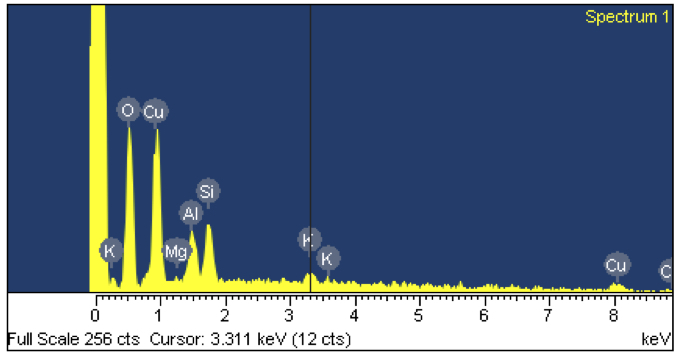
\includegraphics[width=0.6\linewidth]{HKI_nat_az_EDS_site2_spectrum1_050521_spectrumimage}
\caption[Point spectrum: HKI natural azurite]{Point spectrum: HKI natural azurite}
\label{fig:hki_eds_spectrum}
\end{figure}

\begin{figure}[H]
\centering
  \includegraphics[width=0.5\linewidth]{HKI_nat_az_EDS_site2_spectrum1_050521_semimage}
\caption[SEM image showing point spectrum sample location: HKI natural azurite]{SEM image showing point spectrum sample location: HKI natural azurite}
\label{fig:hki_eds_sem_image}
\end{figure}

\begin{table}[H]
\caption{HKI natural azurite: EDS quantitative data}
\centering
\label{table:hki_ratios}
\begin{tabular}{c c}
\toprule
\multicolumn{2}{c}{HKI natural azurite} \\
\midrule
Cu:O & Si:O \\
\midrule
0.0104 & 0.2152 \\
0.2558 & 0.0465 \\
0.0114 & 0.2906 \\
0.0040 & 0.1816 \\
0.3498 & 0.1667 \\
0.0251 & 0.3351  \\
0.0097 & 0.2499 \\
0.0060 & 0.1696 \\
\bottomrule
\end{tabular}
\end{table}

EDS mapping data is shown in \textit{Figures \ref{fig:hki_map1}}. This shows that copper and oxygen abundance is highly correlated, and that Cu intensity makes up only approximately 50\% of the mapped area. Carbon distribution appears random, as does potassium and magnesium. Iron appears to be correlated with oxygen, suggesting the presence of some form of iron oxide in low abundance. 

Silicon is correlated to both oxygen and aluminium in most areas in which it is present, with one area showing a silicon/oxygen containing compound that lacks aluminium. There is no apparent link between SEM morphology and elemental composition, and smaller surface particles are not elementally distinct from the larger substrate they rest on. Interestingly, the sample consists of as much or more copper-free content as copper-containing content, and only one of eight point spectra shows the expected Cu:O atomic ratio. 

\begin{figure}[H]
\centering
  \includegraphics[width=0.9\linewidth]{HKI_nat_az_EDS_map1_050521_imgs}
\caption[EDS mapping data: HKI natural azurite]{EDS mapping data: HKI natural azurite}
\label{fig:hki_map1}
\end{figure}


% ************************************************    Az1    ********************************************************************

C, O, Cu, Al, and Si were detected in sample Az 1. \textit{Table \ref{table:az1_ratios}} shows calculated Cu:O atomic ratios from point spectra. The average Cu:O ratio value is 0.3031 (SD = 0.0631). This is on the lower end of expected ratio values for azurite, though several ratio values are very close to that expected. The Si:O ratios were very consistent, averaging around 0.04, and the average Si:Al ratios were also quite consistent, averaging 1.44, though silicon was not present in all point spectra.

\begin{table}[H]
\caption{Az 1: EDS quantitative data}
\centering
\label{table:az1_ratios}
\begin{tabular}{c}
\toprule
Az 1, azurite \\
\midrule
Cu:O \\
\midrule
0.3150 \\
0.3236 \\
0.2920 \\
0.2018 \\
0.3969 \\
0.2893 \\
\bottomrule
\end{tabular}
\end{table}

\textit{Figure \ref{fig:az1_map1}} shows mapping data for sample Az 1. Copper and oxygen are spatially correlated. Detection of zinc occurs in the same areasof the sample as copper, and as these two elements have closely overlapping peaks, this attribution is interpreted as in error. Carbon appears in areas where the EDS carbon-based tab is exposed.

Silicon and aluminium appear concurrently in some smaller areas of the sample, suggesting that an aluminosilicate is present in association with the copper carbonate. Silicon also appears independent of aluminium, strongly correlated with oxygen, which suggests quartz. 

\begin{figure}[H]
\centering
  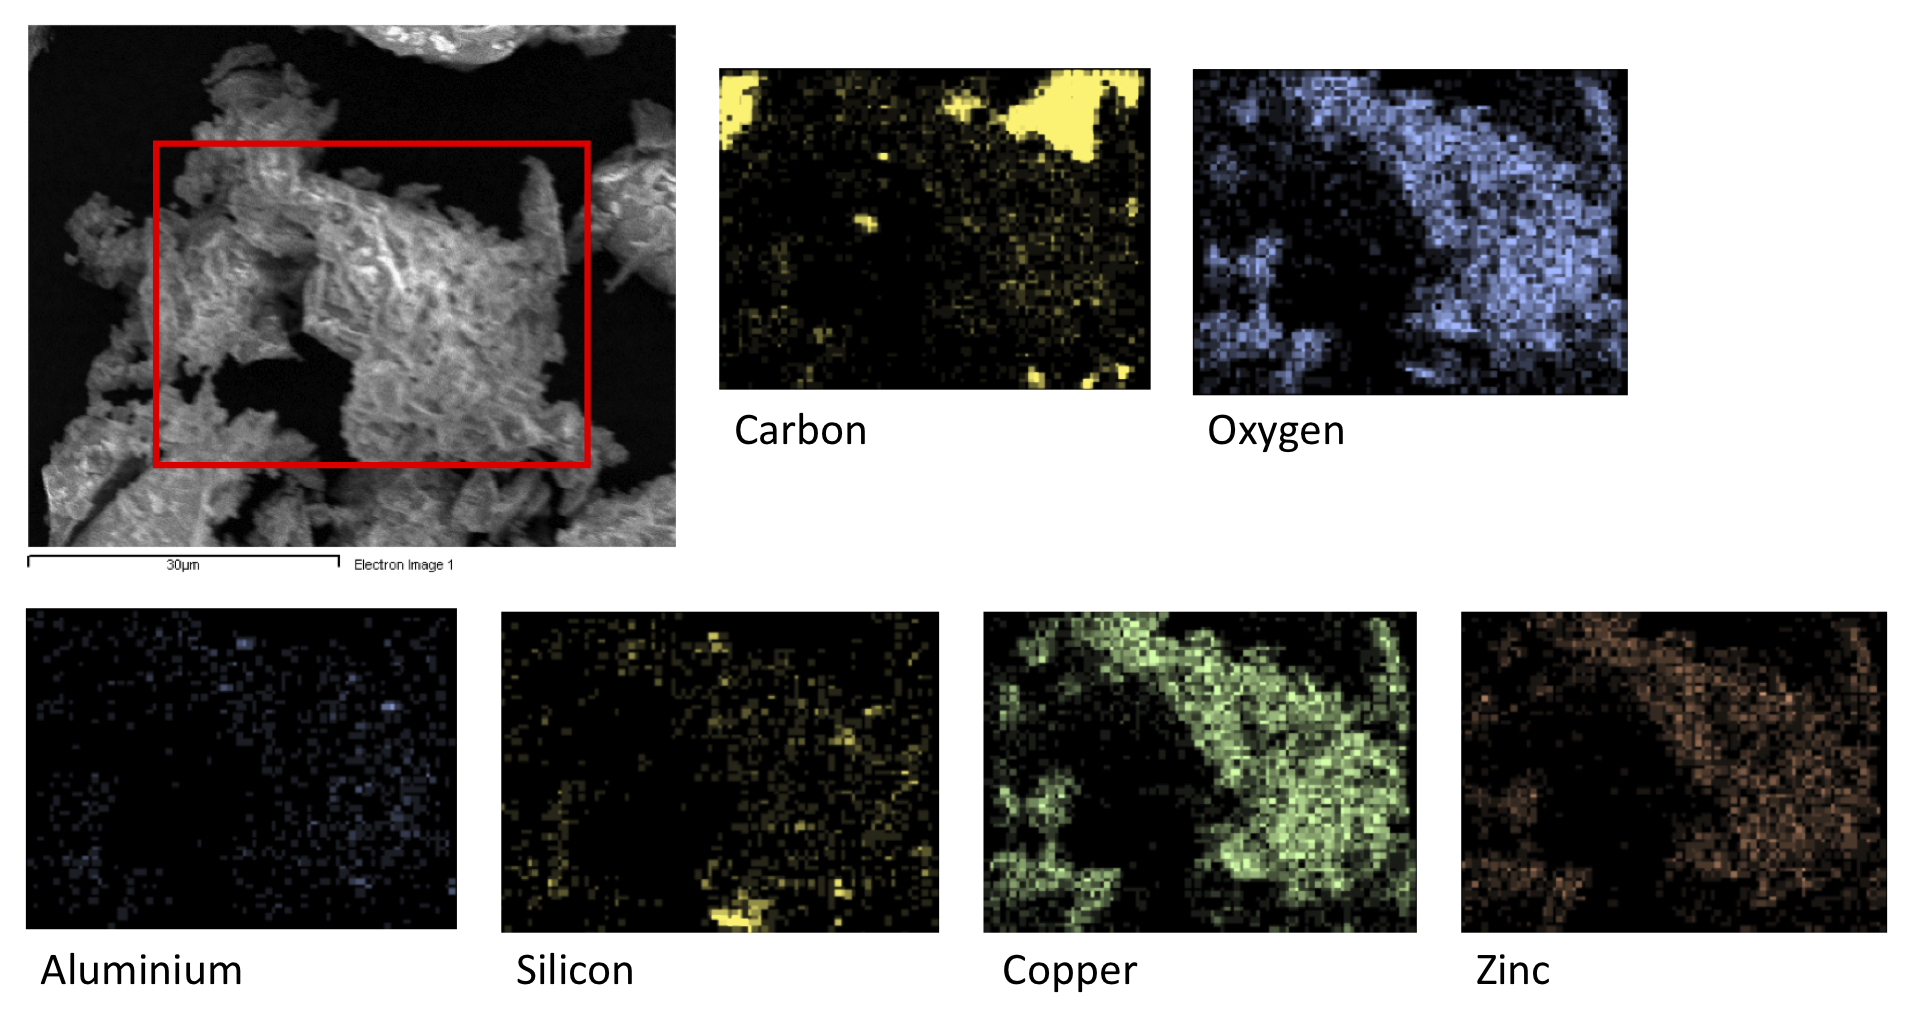
\includegraphics[width=0.9\linewidth]{Az1_EDS_map2_250221_img}
\caption[EDS mapping data: Az 1]{EDS mapping data: Az 1}
\label{fig:az1_map1}
\end{figure}


% ************************************************    Az2    ********************************************************************

C, O, Cu, and Si were detected in sample Az 2. Cu:O ratios calculated from point spectra show inconsistent values, 0.2699 and 0.3897 (\textit{Table \ref{table:az2_ratios}}). However, the calculated Si:O ratios at the same locations do not explain the fluctuation; the ratio of 0.0198 Si:O is far too small to indicate a silicon oxide type mineral.

\begin{table}[H]
\caption{Az 2: EDS quantitative data}
\centering
\label{table:az2_ratios}
\begin{tabular}{c c}
\toprule
\multicolumn{2}{c}{Az 2, azurite} \\
\midrule
Cu:O & Si:O \\
\midrule
0.2699 & 0.0198 \\
0.3897 & 0 \\
\bottomrule
\end{tabular}
\end{table}

\textit{Figure \ref{fig:az2_map1}} shows that while copper and oxygen are highly correlated across the sample map, silicon and carbon are randomly distributed. This suggests that silicon is present as a trace element rather than a major component of the pigment, and this is supported by the low Si:O ratios calculated from the point spectra. This means that the variation in Cu:O atomic ratio values must be due to a factor other than intensity due to another mineral present.

\begin{figure}[H]
\centering
  \includegraphics[width=0.9\linewidth]{Az2_EDS_map1_250221_imgs}
\caption[EDS mapping data: Az 2]{EDS mapping data: Az 2}
\label{fig:az2_map1}
\end{figure}

% ************************************************    AzMag    ********************************************************************

The elements detected in sample AzMag are C, O, Cu, Si, and Ca. The calculated Cu:O ratios, shown in \textit{Table \ref{table:azmag_ratios}}, are 0.1786 and 0.3404. These are not consistent: 0.3404 is very close to the expected ratio for basic copper carbonates, but 0.1786 is well outside the expected range. Silicon is present at very low levels (approximate Si:O ratio = 0.01), and does not explain this variation. Calcium is present in the first sample with a ratio of 0.1012, which is significant. It is possible that a calcium containing mineral is present throughout this sample, a conclusion supported by mapping data.

\begin{table}[H]
\caption{AzMag: EDS quantitative data}
\centering
\label{table:azmag_ratios}
\begin{tabular}{c }
\toprule
AzMag, azurite \\
\midrule
Cu:O \\
\midrule
0.1786 \\
0.3404 \\
\bottomrule
\end{tabular}
\end{table}

\textit{Figure \ref{fig:azmag_map1}} shows mapping data for sample AzMag. Silicon and carbon show lower intensity than copper and oxygen, but all four are closely correlated spatially. Calcium was not detected in the mapping data.

\begin{figure}[H]
\centering
  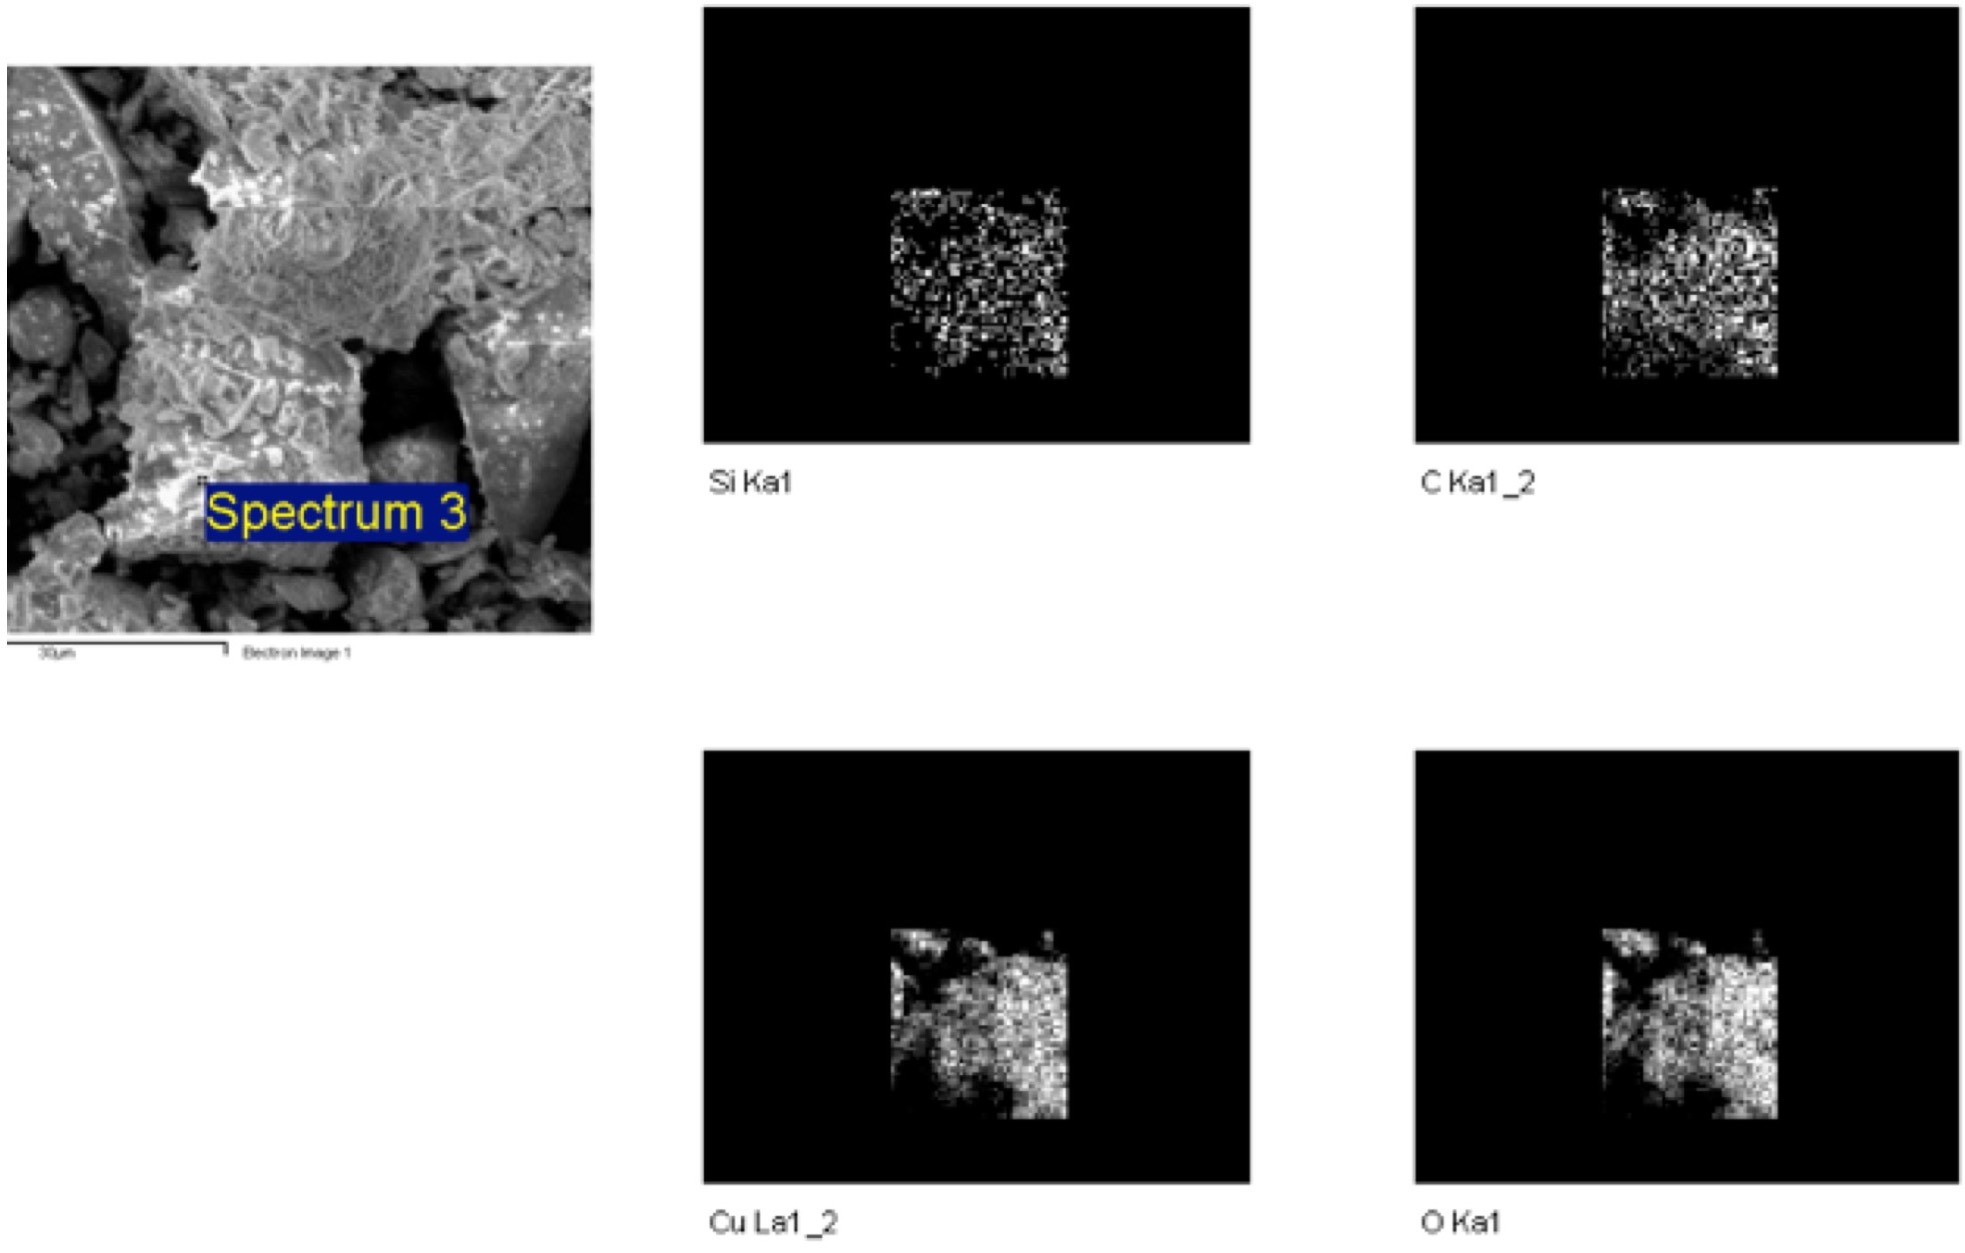
\includegraphics[width=0.9\linewidth]{AzMag_EDS_map1_260221_imgs}
\caption[EDS mapping data: AzMag]{EDS mapping data: AzMag}
\label{fig:azmag_map1}
\end{figure}


% ************************************************    AzOp    ********************************************************************

C, O, Cu, Al, and Si are detected in sample AzOp. Atomic ratios are shown in \textit{Table \ref{table:azop_ratios}}. Cu:O ratios calculated from point spectra are very low in sample AzOp, while those of Si:Al and Si:O are relatively high compared to other samples. This suggests that the sample contains other minerals such as quartz or aluminum silicate may be present, though the calculated atomic ratios do not fit empirical formulae so it is not possible to allow determination of these minerals from EDS data alone.

\begin{table}[H]
\caption{AzOp: EDS quantitative data}
\centering
\label{table:azop_ratios}
\begin{tabular}{c c c}
\toprule
\multicolumn{3}{c}{AzOp, azurite} \\
\midrule
Cu:O & Si:Al & Si:O \\
\midrule
0.2330 & 1.2572 & 0.1051 \\
0.2062 & 1.1140 & 0.0753 \\
\bottomrule
\end{tabular}
\end{table}

\textit{Figure \ref{fig:azop_map1}} shows mapping data for sample AzOp. Copper and oxygen are clearly correlated, and carbon is somewhat correlated to copper and oxygen; all expected for a basic copper carbonate. However, areas also show significant correlation between silicon and oxygen. Silicon is abundant all over the sample. Mapping data does not show aluminium intensity, surprisingly. 

\begin{figure}[H]
\centering
  \includegraphics[width=0.9\linewidth]{AzOp_EDS_map1_260221_imgs}
\caption[EDS mapping data: AzOp]{EDS mapping data: AzOp}
\label{fig:azop_map1}
\end{figure}

% ************************************************    Fitz1    ********************************************************************

C, O, Cu, Al (mapping only), Si, and Ca were detected in sample Fitz 1. Atomic ratios are shown in \textit{Table \ref{table:fitz1_ratios}}. Given that Fitz 1 is a synthetic pigment, it is reasonable to hypothesize that it would contain only carbon, copper, and oxygen and show fairly consistent Cu:O ratios across point spectra. Surprisingly, low levels of silicon and calcium were detected, and Cu:O ratios range from 0.1366 (well below the expected ratio for a basic copper carbonate) to 0.3314 (approximately the expected ratio for a basic copper carbonate). Furthermore, the chemical variation is interesting when compared to the morphological consistency observed.

\begin{table}[H]
\caption{Fitz 1: EDS quantitative data}
\centering
\label{table:fitz1_ratios}
\begin{tabular}{c c c}
\toprule
\multicolumn{3}{c}{Fitz 1, blue verditer} \\
\midrule
Cu:O & Ca:O & Si:O \\
\midrule
0.2316 & 0.1555 & 0 \\
0.3115 & 0 & 0.0122 \\
0.1366 & 0.2510 & 0 \\
0.3314 & 0 & 0.0085 \\
\bottomrule
\end{tabular}
\end{table}

\textit{Figure \ref{fig:fitz1_map1}} shows mapping data for sample Fitz 1. Copper is spatially correlated with some areas of oxygen intensity, as is carbon. Calcium appears randomly distributed all over the mapped area. Silicon appears with oxygen in several spots with very high intensity, and aluminium and silicon also appear correlated.

\begin{figure}[H]
\centering
  \includegraphics[width=0.9\linewidth]{Fitz1_EDS_map1_030321_imgs}
\caption[EDS mapping data: Fitz 1]{EDS mapping data: Fitz 1}
\label{fig:fitz1_map1}
\end{figure}

% ************************************************    KE3    ********************************************************************

The elements detected in sample KE 3 are C, O, Cu, Ca, and Si (mapping only). \textit{Table \ref{table:ke3_ratios}} shows the Cu:O and Ca:O ratios from point spectra. While the first ratio value for Cu:O is as expected for a basic copper carbonate, the second is much lower and outside the expected range. This correlates with a much larger Ca:O ratio, suggesting that some particles in the sample may be calcium oxide rather than copper carbonate.

\begin{table}[H]
\caption{KE 3: EDS quantitative data}
\centering
\label{table:ke3_ratios}
\begin{tabular}{c c}
\toprule
\multicolumn{2}{c}{KE 3, light verditer bice} \\
\midrule
Cu:O & Ca:O \\
\midrule
0.3411 & 0.0069 \\
0.2052 & 0.1108 \\
\bottomrule
\end{tabular}
\end{table}

\textit{Figure \ref{fig:ke3_map1}} shows mapping data for sample KE 3. Silicon appears in mapping data sporadically but not in point spectra. Copper is correlated with oxygen, as is calcium to some extent.

\begin{figure}[H]
\centering
  \includegraphics[width=0.9\linewidth]{KE3_EDS_map1_050321_imgs}
\caption[EDS mapping data: KE 3]{EDS mapping data: KE 3}
\label{fig:ke3_map1}
\end{figure}

% ************************************************    KE4    ********************************************************************

C, O, Cu, and Ca were detected in sample KE 4. Point spectra show calculated Cu:O ratios (\textit{Table \ref{table:ke4_ratios}}) that, while slightly low, are within range of that expected for azurite (particularly the second ratio, 0.3381). The calculated Ca:O ratios are very low.

\begin{table}[H]
\caption{KE 4: EDS quantitative data}
\centering
\label{table:ke4_ratios}
\begin{tabular}{c c}
\toprule
\multicolumn{2}{c}{KE 4, blue bice} \\
\midrule
Cu:O & Ca:O \\
\midrule
0.2703 & 0.0660 \\
0.3381 & 0.0095 \\
\bottomrule
\end{tabular}
\end{table}

\textit{Figure \ref{fig:ke4_map1}} shows mapping data for sample KE 4. Copper and oxygen, as observed in other samples, are spatially correlated. Carbon is also correlated to copper and oxygen. Calcium is correlated to oxygen as well, only in areas absent of copper, suggesting some form of calcium oxide is present.

\begin{figure}[H]
\centering
  \includegraphics[width=0.9\linewidth]{KE4_EDS_map1_030321_imgs}
\caption[EDS mapping data: KE 4]{EDS mapping data: KE 4}
\label{fig:ke4_map1}
\end{figure}

% ************************************************    KE5    ********************************************************************

The elements detected in sample KE 5 are C, O, and Cu. The average ratio of Cu:O is 0.3150 (standard deviation = 0.0311), and all sampled atomic ratios are shown in \textit{Table \ref{table:ke5_ratios}}. While this value is lower than expected, it is within reason given the possible error in quantitative determination of oxygen.

\begin{table}[H]
\caption{KE 5: EDS quantitative data}
\centering
\label{table:ke5_ratios}
\begin{tabular}{c}
\toprule
KE 5, blue verditer \\
\midrule
Cu:O \\
\midrule
0.3371 \\
0.3284 \\
0.2794 \\
\bottomrule
\end{tabular}
\end{table}

% ************************************************    Ma1    ********************************************************************

The elements detected in sample Ma 1 are C, O, and Cu. \textit{Figure \ref{fig:ma1_map1}} shows mapping data from sample Ma 1. Zinc is also shown at low abundance in mapping data, though this is likely intensity due to copper since the peaks of copper and zinc overlap. There is correlation between carbon, oxygen, and copper, and the Cu:O ratio is 0.3675, expected for a basic copper carbonate compound. 

\begin{figure}[H]
\centering
  \includegraphics[width=0.9\linewidth]{Ma1_EDS_map1_250221_imgs}
\caption[EDS mapping data: Ma 1]{EDS mapping data: Ma 1}
\label{fig:ma1_map1}
\end{figure}

% ************************************************    KE1a    ********************************************************************

C, O, Cu, and Ca were detected in sample KE 1a. Calcium is present in relatively low levels, and is likely a trace element rather than a major component of the pigment. The measured Cu:O ratios (\textit{Table \ref{table:ke1a_ratios}}) are within the range expected for a basic copper carbonate.

\begin{table}[H]
\caption{KE 1a: EDS quantitative data}
\centering
\label{table:ke1a_ratios}
\begin{tabular}{c c}
\toprule
\multicolumn{2}{c}{KE 1a, green bice} \\
\midrule
Cu:O & Ca:O \\
\midrule
0.3483 & 0.0086 \\
0.3622 & 0.0066 \\
\bottomrule
\end{tabular}
\end{table}

% ************************************************    KE2    ********************************************************************

C, O, Cu, and Si (mapping only) were detected in sample KE 2. The measured Cu:O ratios (\textit{Table \ref{table:ke2_ratios}} are within the range expected for a basic copper carbonate, and are among the highest measured of any samples.

\begin{table}[H]
\caption{KE 2: EDS quantitative data}
\centering
\label{table:ke2_ratios}
\begin{tabular}{c}
\toprule
KE 2, green verditer \\
\midrule
Cu:O \\
\midrule
0.3724 \\
0.3944 \\
\bottomrule
\end{tabular}
\end{table}

\textit{Figure \ref{fig:ke2_map1}} shows mapping data for sample KE 2. Carbon is sparsely distributed, and there are areas without any elements detected. Silicon, which is not detected in point spectra, is present in low levels. Copper and oxygen are clearly correlated, as expected.

\begin{figure}[H]
\centering
  \includegraphics[width=0.9\linewidth]{KE2_ES_map1_040321_imgs}
\caption[EDS mapping data: KE 2]{EDS mapping data: KE 2}
\label{fig:ke2_map1}
\end{figure}


All three green samples (Ma 1, KE 1a, and KE 2) show Cu:O atomic ratios that very closely match the expected ratios for both azurite and malachite. The chemical formula for green verditer is as yet unproven, and the margin of error on quantitative analysis is not able to distinguish between a 2:5 and a 3:8 Cu:O ratio. It is clear that there is minimal trace mineral present in all these samples, and that atomic ratios support identification as basic copper carbonates.

%       *****************************

The historical cross section is significantly more complex than the powder samples, both natural and synthetic. Mapping data for the cross section collected on both the JEOL and TESCAN SEM-EDS instruments are presented in \textit{Figures \ref{fig:xsection_map1}} and \textit{Figure \ref{fig:xsection_map2}}. Azurite and verditer pigments are only two components of the sample. The cross section consists of three visually distinct layers, but EDS mapping data shows that layers A and B (in \textit{Figure \ref{fig:hki_crossec_explanation}}) are chemically comparable. The visual difference is likely due to the higher intensity of lead containing components in layer B. 

This sample was carbon-coated prior to analysis, so carbon is present across the entire sample surface. Oxygen is also distributed across the entirety of the cross section, which is expected as many common pigments are metal carbonates or metal oxides and any organic binder components will also contain oxygen. Calcium, aluminium, and silicon are also detected over the entire area of the cross section, with some map data showing correlation between aluminum and silicon. It is likely that an aluminosilicate is present in association with one or more pigments. Calcium-based ground layers are commonly observed, and a material such as limestone could contain Ca, Si, and Al as well as potassium, also detected in the cross section. Potassium is observed in the natural azurite sample from the HKI, which might suggest it is also a marker that could be used to evaluate the nature of azurite pigments.

That said, there is also evidence that aluminosilicates are present as distinct components, as observed in \textit{Figure \ref{fig:xsection_map2}} where silicon and aluminium are observed to be present in precisely localised areas. Calcite is a common mineral associated with azurite and is observed in almost all powder samples, natural and artificial. Calcium carbonates as well as aluminosilicates including kaolinite were also both commonly used as paint extenders, white particles mixed with coloured pigments to lower their cost to produce.~\autocite{Townsend}

Magnesium, lead, and copper are localised to areas of the sample that correspond with distinct pigment particles or aggregates as discussed above. Given the lack of chromium present as well as the colour of the cross sectional layers, the lead pigment present is suggested to be lead white, a basic Lead(II) carbonate that occurs as a mineral called cerussite. While cerussite may occur in association with natural azurite,\autocite{Aru} the abundance of lead and the lack of overlapping areas of lead and copper detected by EDS suggests that lead white was employed as a pigment mixed with the blue azurite.

Magnesium oxides have been used historically as pigments, most importantly \textit{terre verte} or green earth which is a mixture of an iron silicate with a magnesium-containing clay. The low abundance of iron across the sample discourages the assignment of magnesium to terre verte, and therefore, magnesium-based minerals associated with azurite or cerussite must be considered as an explanation. Additionally, magnesium may be present as mica or another common mineral. Iron is detected sporadically across the cross section, which suggests that it is present as a trace element. Arsenic is suggested in one EDS map (\textit{Figure \ref{fig:xsection_map2}}), and this must be evaluated further. \textit{Figure \ref{fig:xsection_map2}} shows mapping data collected from the TESCAN SEM instrument. The magnification is approximately 2000x here. Apart from the detection of arsenic (possibly in association with lead), this map confirms the results acquired on the JEOL instrument.


Quantitative analysis of copper containing areas of the sample shows a Cu:O ratio of, on average, 0.217. This is lower than the expected ratio for azurite/blue verditer. Also detected in these areas are significant levels of iron and lead, indicating that there may be impurities in the blue pigment particles (iron) and/or contribution from the three dimensional structure of the paint mixture containing azurite and lead white. At lower levels there is also silicon and magnesium detected, which may be due to impurities as well. 

This data demonstrates the complexity of analysis of samples consisting of a mixture of different pigments that are also each composed of, potentially, several minerals.

%O, Cu, Ca, Pb, Mg, Al, Si, K, Fe ( map only: As??)

%Darkest: Mg on mapping (low atomic number)
%Lightest: Lead, fine powder, widely distributed through one of the laters, likely mixed with Cu to make a lighter color (lead white)
%Moderate: Copper
%Darker layer shows relatively more Si in mapping

\begin{figure}[H]
\centering
  \includegraphics[width=0.9\linewidth]{hki_cross_section_eds_analysis_250621_site1_map1}
\caption[EDS mapping data: historic cross section, JEOL SEM]{EDS mapping data: historic cross section, JEOL SEM}
\label{fig:xsection_map1}
\end{figure}

\begin{figure}[H]
\centering
  \includegraphics[width=0.9\linewidth]{HKI_cross_section_Site 7_2021-06-30_15-23-55}
\caption[EDS mapping data: historic cross section, TESCAN SEM]{EDS mapping data: historic cross section, TESCAN SEM}
\label{fig:xsection_map2}
\end{figure}

\subsection[Summary of EDS results]{Summary of EDS results}

\textit{Table \ref{table:eds_data_summary}} summarizes the detected elements and average Cu:O ratios for copper-containing point spectra collected from each reference sample. Unsurprisingly, natural azurite samples showed a much greater diversity of elements than synthetic samples. Most samples including synthetic verditers contained calcium, suggesting that it is present in the industrial synthetic process and incorporated into the product. Cu:O ratios, on the other hand, were not diagnostic for sample origin, consistent across all samples within error. For sample Fitz 1, two Cu:O ratios are presented as several points sampled showed large Ca:O ratios that led to a low Cu:O average. The larger Cu:O ratio excludes these points.

\begin{table}[H]
\caption{Summary of EDS data results: reference samples}
\centering
\label{table:eds_data_summary}
\begin{tabular}{c c c}
\toprule
Sample & Detected elements & Cu:O ratio $\pm$ SD \\
\midrule
HKI natural azurite & C, O, Cu, Si, Al, Mg, Ca, K, Fe & 0.3028 $\pm$ 0.0664 \\
Az 1 & C, O, Cu, Si, Al & 0.3031 $\pm$ 0.0631 \\
Az 2 & C, O, Cu, Si & 0.3298 $\pm$ 0.0847 \\
AzMag & C, O, Cu, Si, Ca & 0.2595 $\pm$ 0.1144 \\
AzOp & C, O, Cu, Si, Al  & 0.2196 $\pm$ 0.0190 \\
Fitz 1 & C, O, Cu, Si, Ca & \vtop{\hbox{\strut 0.2528 $\pm$ 0.0886}\hbox{\strut 0.3215 $\pm$ 0.0141}} \\    
KE 3 & C, O, Cu, Ca & 0.2732 $\pm$ 0.0961 \\
KE 4 & C, O, Cu, Ca & 0.3042 $\pm$ 0.0479 \\
KE 5 & C, O, Cu & 0.3150 $\pm$ 0.0311 \\
Ma 1 & C, O, Cu & \textemdash \\
KE 1a & C, O, Cu, Ca & 0.3553 $\pm$ 0.0098 \\
KE 2 & C, O, Cu & 0.3834 $\pm$ 0.0156 \\
Cross section & C, O, Cu, Si, Al, Mg, Ca, K, Fe, Pb, As & \textemdash \\
\bottomrule
\end{tabular}
\end{table}



% *******************************************************************************************************************************
% *******************************************************************************************************************************
% *******************************************************************************************************************************

\section[Raman Data]{Raman Data}
\label{section3.3}

\textit{Figure \ref{fig:label_raman}} shows Raman spectra of samples Az1 (blue) and Ma1 (green). The spectrum from Az1 was collected from a bright blue particle, while the spectrum from Ma1 was collected from the fine green bulk particles. Both therefore are representative of the component of the pigment responsible for the colour rather than of another mineral impurity. Peak centers are labelled. 

Hydroxyl stretching bands are reported by Frost et. al. for azurite at 3453 and 3427 cm\textsuperscript{-1} and for malachite at 3468 and 3386 cm\textsuperscript{-1}.~\autocite{Frost} These bands are not shown here, but were observed. Mattei et. al. note that bands below 600 cm\textsuperscript{-1} are due to CuO vibrations and bands from 600 to 1600 cm\textsuperscript{-1} are due to carbonate vibrations.~\autocite{Mattei}

The Raman spectra shown in \textit{Figure \ref{fig:label_raman}} agree very closely with the literature peak locations.~\autocite{Mattei,Frost,Bicchieri} The technique is capable of identifying azurite and malachite (or their synthetic analogues).

\begin{comment}
azurite
Frost: $v1    v2_Sym  v2_Antisym   v3_B2   v3_A1    v4_B2   v4_A1$
       1095   816       834        1419    1430     765     739

Bicchieri: 145, 180, 250, 284, 335, 403, 545, 746, 767, 839, 940, 1098, 1432 and 1573 cm

Mattei: 157vw 174vw 182vw 240vw 250vw \textbf{267vw} 282vw 332vw
\textbf{387vw} 402s 542vw \textbf{744vw is shoulder} 768w 840w 937vw 1099m
1422m(sh) \textbf{1433m is shoulder in mine} 1462vw 1582w 3431w

Me: 113 139 180 248 284 330 401 507 541 577 764 836 937 1096 1419 1459 1576


malachite

mattei: \textbf{157m(sh) 171m(sh) 182s 204vw 224vw} 272s 352w 435s 513w
537m 601vw 723vw 753vw 1058w 1101w 1370vw 1463vw
1497s 3380w

frost: $v1    v2_Sym  v2_Antisym   v3_B2   v3_A1    v4_B2   v4_A1$
      1096     816      801       1492     1364     752     717
                                  1514     1423

Me: 120 144 153 168 180 222 269 352 433 509 533 565 598 720 749
\end{comment}

Spectra comparing the reference azurite and verditer pigments are shown in \textit{Figure \ref{fig:blue_comparison1}}-\textit{\ref{fig:blue_comparison3}}. All spectra are collected from bulk blue or green particles. The Raman spectra of natural samples are compared in \textit{Figure \ref{fig:blue_comparison1}} and \textit{Figure \ref{fig:blue_comparison2}} (alongside KE 4, of ambiguous origin). The Raman spectra of synthetic samples are compared in \textit{Figure \ref{fig:blue_comparison3}}. All green samples are compared in \textit{Figure \ref{fig:green_comparison}}.

Natural azurite samples show consistent peak locations, though intensity ratios vary. Samples Fitz 1, KE 3, KE 4, and KE 5 are also consistent. However, the low frequency region shows variation between natural and synthetic samples. This is the lattice vibration region, and variation suggests that bond structures vary in crystals of natural and synthetic origin.

Green samples varied significantly in the region of 400-600 cm\textsuperscript{-1}, showing a strong peak at either 400 cm\textsuperscript{-1} and 450 cm\textsuperscript{-1} or 430 cm\textsuperscript{-1}. The natural malachite sample Ma 1 also shows additional bands above 500 cm\textsuperscript{-1} that are not clearly observed in the rest. 

These results suggest that although interpretation of mineral Raman spectra is difficult due to the influence of structural variation on spectral bands, this analysis can be used in combination with other methods to support a natural or synthetic origin for a sample. 

\begin{figure}[H]
\centering
\begin{minipage}[t]{\linewidth}
  \centering
  \includegraphics[width=0.9\linewidth]{az1_blue_withlabels}
\hfill
\includegraphics[width=0.9\linewidth]{natural_malachite_graph_labelled}
\hfill
\end{minipage}
\caption[Raman spectra of natural azurite and malachite, peak centers labelled.]{Raman spectra of natural azurite (blue, top) and malachite (green, bottom). Peak centers are labelled.}
\label{fig:label_raman}
\end{figure}

\begin{figure}[H]
\centering
  \includegraphics[width=0.8\linewidth]{hki_az1_az2}
\caption[Raman spectra of blue samples.]{Raman spectra of verditer and azurite samples: HKI natural azurite, Az 1, Az 2. Spectra are offset for clarity.}
\label{fig:blue_comparison1}
\end{figure}

\begin{figure}[H]
  \centering
  \includegraphics[width=0.8\linewidth]{hki_azmag_azop_ke4}
\caption[Raman spectra of blue samples.]{Raman spectra of verditer and azurite samples: HKI natural azurite, AzMag, AzOp, KE 4. Spectra are offset for clarity.}
\label{fig:blue_comparison2}
\end{figure}

\begin{figure}[H]
  \centering
  \includegraphics[width=0.8\linewidth]{fitz1_ke3_ke4_ke5}
\caption[Raman spectra of blue samples.]{Raman spectra of verditer and azurite samples: Fitz1, KE 3, KE 4, KE 5. Spectra are offset for clarity.}
\label{fig:blue_comparison3}
\end{figure}

\begin{figure}[H]
\centering
  \includegraphics[width=0.8\linewidth]{ma1_ke1a_ke1b_ke2}
\caption[Raman spectra of green samples.]{Raman spectra of natural malachite and synthetic green verditer samples: Ma 1, KE 1a, KE 1b, and KE 2. Spectra are offset for clarity.}
\label{fig:green_comparison}
\end{figure}

Several powdered azurite and verditer samples contained particles that differed in colour from the main component, basic copper carbonate. \textit{Figure \ref{fig:label_raman}} shows green and white mineral inclusions in samples Az 2, AzMag, AzOp, KE 4, and KE 5. Several of these spectra are clearly attributable to associate minerals, such as quartz and terre verte (a general term for iron-based green clays, often also containing potassium, magnesium, aluminium, and silicon).~\autocite{ucl_database,cameo_mfa,irug_quartz} Quartz and various clays are reasonable to expect based on known associate minerals.

Two green inclusions in blue samples show strong bands that correlate to azurite and malachite. Malachite is a common associate mineral of azurite, as well as a degradation product. From the historical record of verditer production, it is known that crystals may vary in colour from blue to green depending on environmental conditions, and this may also explain the green colour of a particle that appears to be azurite in sample AzMag. It is reasonable to think that natural samples may show colour variations. 

Two white inclusions, in samples Az 2 and AzOp, are not yet identified. These spectra are not attributable to any common associate minerals or known white pigments. The confocal illumination system may make samples appear white if they are highly reflecting, though likely metallic minerals have also been excluded. The strong bands at 373, 823, and 878 cm\textsuperscript{-1} in the spectrum collected from Az 2 are suggestive of Al-O and Si-O vibrational modes in aluminosilicates, but the diversity of this mineral group and large number of possible assignments in these regions makes conclusive identification difficult.~\autocite{Culka} One challenge present in identifying these associate minerals is that their damage threshold is often lower than that of azurite or malachite, requiring lower laser powers and shorter acquisition times in order to avoid destruction.

\begin{figure}[H]
\centering
\begin{minipage}[t]{\linewidth}
  \centering
  \includegraphics[width=0.9\linewidth]{green_inclusions}
\hfill
\includegraphics[width=0.9\linewidth]{white_inclusions}
\hfill
\end{minipage}
\caption[Raman spectra of green and white mineral inclusions in azurite.]{Raman spectra of green (top) and white (bottom) mineral inclusions in azurite. Reference azurite and malachite spectra are shown for comparison purposes, and spectra are scaled and offset for clarity. Identifiable spectra are labelled, and bands attibutable to copper carbonate and malachite are highlighted for ease of comparison to references.}
\label{fig:label_raman}
\end{figure}

Analysis of resin embedded samples, including historical cross sections, proved difficult using the confocal Raman system. \textit{Figure \ref{fig:fluor_example_graph}} shows two spectra collected using an excitation wavelength of 532 nm from the surface of the historical cross section sample. Azurite is clearly present in one spectrum, shown in black, with a strong band at 400 cm\textsuperscript{-1} (band highlighted in blue). Cerussite (lead white) is present in both spectra (highlighted in grey). Broac baselines were subtracted but it is apparent from the presence of a regular scalloped peak shape that additional fluorescence is present. Analysis of the polyester resin without pigment present shows that these bands are from resin contributions, though similar fluorescense has also appeared as discussed previously in spectra of impurities in powdered azurite and verditer samples. 

These bands are present in all spectra collected from the historical cross section sample, and the signal is strong enough to mask contributions from smaller azurite peaks and is comparable in intensity to contributions from cerussite, a major component of the cross section along with azurite. This clearly poses a problem for detection of variation in pigments and introduces uncertainty into the results.

\textit{Figure \ref{fig:contours_xsection}} shows contour plots of azurite peak intensity (left) and integrated peak area (right) across a 10 x 10 spectrum map of an area of the cross section. The undertainty introduced by the strong resin bands is apparent, as peak area and peak intensity do not indicate azurite particles are present in the same areas of the map. This is due to varying contributions from the underlying fluorescence band that are difficult to subtract without introducing additional errors into the analysis.

\begin{figure}[H]
\centering
  \includegraphics[width=0.9\linewidth]{fluor_example_graph}
\caption[Raman spectra of historical cross section]{Raman spectra of two points on historical cross section, blue area. The semicircular repeated peak formation observed is due to fluorescence from the resin (contribution from non-azurite pigment particles and organic binder is also possible). The major azurite (blue) and cerussite (grey) peaks are highlighted on the graph and spectra are offset for clarity.}
\label{fig:fluor_example_graph}
\end{figure}


\begin{figure}[H]
\centering
\begin{minipage}{.45\textwidth}
  \centering
  \includegraphics[width=\linewidth]{050721map400intensities}
\end{minipage}
\begin{minipage}{.45\textwidth}
  \centering
  \includegraphics[width=\linewidth]{050721map400areas}
\end{minipage}
\caption[Contour maps, azurite Raman intensity in historical cross section]{Contour maps show the Raman intensity as: \textbf{left)} 400 cm\textsuperscript{-1} peak intensity and \textbf{right)} 400 cm\textsuperscript{-1} integrated peak area. X and Y axes map to locations on the sample surface where spectra were collected, in total 10 x 10 = 100 spectra.}
\label{fig:contours_xsection}
\end{figure}

The 473 nm excitation wavelength was also tested to determine whether the fluorescence would be mitigated by shifting the excitation frequency. This was determined not to resolve the issue, with fluorescence and sample bands showing a similar increase in intensity at 473 nm. It may be possible to generate sample spectra without fluorescence by moving to the anti-Stokes spectrum rather than the Stokes spectrum, as fluorescence is not possible in the anti-Stokes region. However, this may come at the cost of overall intensity and signal-to-noise strength.

%az1_blue_withlabels
%Ma1_labels

%green_pigments_all_labels
%blue_HKI_AzMag_AzOp_Ke4
%blue_HKI_Az1_Az2_labels
%blue_Fitz1_Ke5_Ke3_labels
%blue_Fitz1_Ke5_Ke3_Ke4_labels


% *******************************************************************************************************************************
% *******************************************************************************************************************************
% *******************************************************************************************************************************

\section[AFM Data]{AFM Data}
\label{section3.4}

%      HKI natural azurite

AFM images recorded in tapping mode capture height, deflection, and phase variation across the sample surface. While height measurements are self-explanatory, phase and deflection measurements record variations in mechanical and chemical properties that are not easily deconvoluted or quantified. Deflection refers to the displacement of the tip with interaction with the surface, while the phase shift refers to the difference between the oscillation frequency of the tip initially and after interaction with the surface.~\autocite{iscpi} The phase shift and deflection measurements are therefore affected by changes in the tip interaction with the surface such as adherence or repulsion. 

Height effects can also appear in phase and deflection maps, appearing as intensity changes that change direction as the tip passes over a structure on the surface of the sample. These will appear, for instance, as a high deflection voltage or phase shift on the left side of the structure and a low deflection voltage or phase shift on the right side as the tip scans from left to right. This is due to changing the contact area of the tip with the sample as it approaches a change in topography.~\autocite{iscpi} 

\textit{Figure \ref{fig:afm_hki_nataz_height_phase_1}} shows height and phase shift maps of an 80 x 80 $\mu$m area of sample HKI natural azurite. The surface texture is very dense and shows some small circular particles, shown in the height and phase shift maps. Tip dragging on the surface causes distortions to the image. 

Additional AFM and AFM-IR images are presented in Appendix A, Supplemental data. Although this method has great potential in the analysis of highly polished or microtomed mineral samples, preparation capability to date does not allow sufficiently flat surfaces for clear imaging, leading to images with instrumental artefacts obscuring information about the sample. In particular, deflection images showed primarily instrument artefacts. Additionally, infrared measurements on the instrument currently are not reliable. This technique may be revisited in the future as time and need allow.

\begin{figure}[H]
\centering
\begin{minipage}{.45\textwidth}
  \centering
  \includegraphics[width=\linewidth]{hki_nataz_tapping_mode_150721_height_1}
\end{minipage}
\begin{minipage}{.45\textwidth}
  \centering
  \includegraphics[width=\linewidth]{hki_nataz_tapping_mode_150721_phase_1}
\end{minipage}
\caption[Height and phase maps, HKI natural azurite]{Height and phase maps, HKI natural azurite, 80 x 80 $\mu$m.}
\label{fig:afm_hki_nataz_height_phase_1}
\end{figure}


\section[Battle of Spurs data]{\textit{Battle of Spurs} data}
\label{section3.5}

Areas of visible blue particles in sample 1259.20 were studied by confocal Raman spectroscopy to confirm their identity as azurite. An example sample spectrum is shown in \textit{Figure \ref{fig:raman_1259-20}}. Although the sample spectra suffer from low intensities compared to fluorescence from the surrounding resin, the characteristic band at 400 cm\textsuperscript{-1} is visible, confirming the presence of azurite.

\begin{figure}[H] %%%%%%
\centering
  \includegraphics[width=0.8\linewidth]{1259.20_blue_overpaint}
\caption[Raman spectral data, 1259.20]{Raman spectral data: sample 1259.20. An azurite reference spectrum (blue line) is shown as a comparison to sample 1259.20 (red circles). The spectral data from 1259.20 is smoothed using an FFT filter (black line). Spectra are off-set for clarity.}
\label{fig:raman_1259-20}
\end{figure}

